% =====================================================================
%  Research-paper version (~20 pages) of the Microfluidics term project
%  Compile:  latexmk -pdf paper.tex
% =====================================================================
\documentclass[11pt,a4paper]{article}

\usepackage[T1]{fontenc}
\usepackage[utf8]{inputenc}
\usepackage{lmodern}
\usepackage{microtype}
\usepackage[a4paper,left=22mm,right=22mm,top=22mm,bottom=24mm,headheight=14pt]{geometry}
\usepackage{amsmath,amssymb,mathtools,bm}
\usepackage{graphicx}
\usepackage{booktabs,tabularx,array}
\usepackage{float}
\usepackage[font=small,labelfont=bf,margin=2mm]{caption}
\usepackage{subcaption}
\usepackage[dvipsnames]{xcolor}
\usepackage{siunitx}
\sisetup{separate-uncertainty=true, range-phrase=--, per-mode=symbol}
\usepackage{setspace}
\setstretch{1.12}
\usepackage{enumitem}
\setlist{itemsep=1pt,topsep=3pt}
\usepackage{fancyhdr}
\usepackage{titlesec}
\usepackage[numbers,sort&compress]{natbib}
\usepackage[colorlinks=true,linkcolor=MidnightBlue,citecolor=OliveGreen,urlcolor=MidnightBlue]{hyperref}
\usepackage[capitalise,nameinlink]{cleveref}
\crefname{equation}{Eq.}{Eqs.}

\titleformat{\section}{\normalfont\large\bfseries\color{MidnightBlue}}{\thesection}{0.7em}{}
\titleformat{\subsection}{\normalfont\normalsize\bfseries}{\thesubsection}{0.7em}{}
\titlespacing*{\section}{0pt}{12pt}{5pt}
\titlespacing*{\subsection}{0pt}{9pt}{3pt}

\pagestyle{fancy}
\fancyhf{}
\fancyhead[L]{\small\itshape Shear stress and oxygen transport in a widening Hele-Shaw chip}
\fancyhead[R]{\small Srivastav, Divya, Singal}
\fancyfoot[C]{\small\thepage}
\renewcommand{\headrulewidth}{0.4pt}

\DeclareSIUnit\dyne{dyn}
\DeclareSIUnit\uLmin{\micro\litre\per\minute}
\DeclareSIUnit\dyncm{\dyne\per\centi\metre\squared}
\newcommand{\ulmin}{\si{\uLmin}}
\newcommand{\Csat}{C_{\mathrm{sat}}}
\newcommand{\Cb}{\bar C}
\newcommand{\Cbot}{C_{\mathrm{bot}}}
\newcommand{\Ctop}{C_{\mathrm{top}}}
\newcommand{\qmax}{q_{\max}}
\newcommand{\Km}{K_{m}}
\newcommand{\kp}{k_{\mathrm{PDMS}}}
\newcommand{\taw}{\tau_{w}}
\newcommand{\dd}{\mathrm{d}}
\newcommand{\Pe}{\mathit{Pe}}
\newcommand{\Rey}{\mathit{Re}}
\newcommand{\Da}{\mathit{Da}}
\newcommand{\Bi}{\mathit{Bi}}

\graphicspath{{figures/}}

% ---------------------------------------------------------------- title
\title{\vspace{-8mm}\textbf{Shear Stress and Oxygen Transport in a Widening Hele-Shaw Microfluidic Chip: Numerical Validation and an Analytical Oxygen Model}}
\author{Utkarsh Srivastav (2023CH70715) \quad Divya (2023CH10309) \quad Ishaan Singal (2023CH70545)\\[1mm]
\small Department of Chemical Engineering, IIT Delhi\\
\small Microfluidics (CLL770), term project}
\date{\small November 2026}

\begin{document}
\maketitle
\thispagestyle{fancy}

% ---------------------------------------------------------------- abstract
\begin{abstract}
\noindent
Delon \emph{et al.} (2020) proposed a Hele-Shaw chip whose width grows as $w(x)=w_1L/(L-x)$, so that the wall shear stress on cultured cells falls linearly along the channel. We reproduced their device (\SI{1}{}--\SI{10}{mm} wide, \SI{145}{\micro\metre} high, $L=\SI{50}{mm}$) with steady three-dimensional ANSYS Fluent simulations at 0.22, 1 and \SI{120}{\uLmin}, and compared the results with three levels of lubrication theory: the parallel-plate formula of the paper (T1), its exact side-wall correction (T2) and a two-dimensional model of the full planform (T3). The flow is a Stokes flow: all quantities scale with $Q$ to within \SI{0.08}{\percent}, and $\Delta p=\SI{1.657}{Pa}$ per \ulmin. The published shear ranges are reproduced (\SIrange{0.0102}{0.0014}{\dyncm} against $\sim$\SIrange{0.01}{0.001}{\dyncm} at \SI{0.22}{\uLmin}). At stations S1--S4 the CFD agrees with T1 to $\pm\SI{3.3}{\percent}$, but this agreement is partly a cancellation. The CFD contains the side-wall drag that T1 omits (up to \SI{+9}{\percent}) and lies uniformly \SI{5.2(4)}{\percent} below T2, most probably because there are too few cells across the gap. Offset-free ratios agree with T3 to within \SI{1}{\percent}, including the \SI{+46.5}{\percent} excess over T1 at the outlet corner (S5). The shear is uniform within $\pm\SI{5}{\percent}$ over \SI{70}{}--\SI{91}{\percent} of the width at S1--S4. We then derived an oxygen transport model in which the geometry enters only through the upstream cell area $A(x)=w_1L\ln[L/(L-x)]$, and solved it in closed form. With impermeable walls and illustrative uptake, convection cannot feed the cells below \SI{1.55}{\uLmin}. Anoxia is predicted beyond \SI{13.9}{mm} and \SI{38.7}{mm} at 0.22 and \SI{1}{\uLmin}, exactly in the low-shear region. A \SI{5}{mm} PDMS lid can supply 25 times the uptake and holds the cells at $0.95\,\Csat$. The oxygen results are model predictions that remain to be tested by simulation and experiment.
\end{abstract}

\noindent\textbf{Keywords:} Hele-Shaw flow; wall shear stress; organ-on-chip; lubrication theory; CFD validation; oxygen transport

% =====================================================================
\section{Introduction}

Epithelial and endothelial cells respond to the fluid shear stress (FSS) on their apical surface. Organ-on-chip devices exploit this by culturing cells under flow \citep{BhatiaIngber2014,Zhang2018,Kim2012}. To study the response systematically, a device must expose cells to a known range of shear stresses. The linear-shear chamber of Usami \emph{et al.}~\citep{Usami1993}, adapted to PDMS chips by Delon \emph{et al.}~\citep{Delon2019,Delon2020}, does this in a single channel. A shallow channel whose width increases hyperbolically,
\begin{equation}
w(x)=\frac{w_1L}{L-x},
\label{eq:width}
\end{equation}
carries a wall shear stress that decreases linearly from inlet to outlet. Delon \emph{et al.}\ supported the design formula with CFD and used it to choose regions for imaging the cells.

Two questions remain open. First, how accurate is the design formula? It assumes infinite parallel plates, yet the channel has side walls and ends in a sharp \ang{45} corner. Second, can the cells be supplied with oxygen? Low shear requires low flow, and low flow delivers little oxygen \citep{Place2017,Wagner2011}. In this geometry the lowest shear also occurs downstream, where the medium has already passed over the most cells. A flow simulation alone cannot detect the resulting hypoxia. Perfused PDMS reactors are known to develop axial oxygen gradients despite the permeability of the walls \citep{Mehta2007}.

This paper (i) reproduces the device numerically and validates the CFD against the published results and against a hierarchy of analytical models, and (ii) extends the validated flow to an oxygen transport model with closed-form solutions. Part (i) uses our own simulations. Part (ii) is analytical: an oxygen CFD set-up was prepared but has not been run, and the uptake parameters are illustrative.

% =====================================================================
\section{Device and flow model}

\subsection{Geometry}

The fluid domain (\cref{fig:geometry}) has a uniform height $h=\SI{145}{\micro\metre}$ and four parts in plan view:
\begin{itemize}
\item a straight lead-in, \SI{2}{mm} long and \SI{1}{mm} wide, carrying the inlet;
\item the hyperbolic section, \cref{eq:width}, with $w_1=\SI{1}{mm}$ and $L=\SI{50}{mm}$, up to $x_t=L(1-w_1/w_{\max})=\SI{45}{mm}$ where $w=\SI{10}{mm}$;
\item walls at \ang{45} converging to \SI{1.5}{mm};
\item a \SI{1}{mm} outlet duct.
\end{itemize}
The cells grow on the glass floor ($z=0$); the lid and side walls are PDMS. Stations S1--S5 lie at $x=5$, 15, 25, 35 and \SI{45}{mm}. The local aspect ratio $h/w$ falls from 0.145 at $x=0$ to 0.0145 at S5. The wall half-angle $\arctan[\tfrac12\dd w/\dd x]$ grows from \ang{0.6} to \ang{6.3} at S4, and S5 lies exactly on the corner where the walls turn through \ang{90}.

The reference paper is inconsistent on two dimensions: it quotes $h=150$ and \SI{145}{\micro\metre}, and $L=\SI{5.3}{cm}$. However, its own floor-area integral, $\int_0^{4.5}w\,\dd x=\SI{1.151}{cm^2}$, is reproduced only with $L=\SI{5}{cm}$, which supports our choice of $L=\SI{50}{mm}$. The floor area of the hyperbolic section is
\begin{equation}
A_{\mathrm{cells}}=\int_0^{x_t}w\,\dd x=w_1L\ln\frac{w_{\max}}{w_1}=\SI{115.13}{mm^2}.
\label{eq:area}
\end{equation}

\begin{figure}[t]
\centering
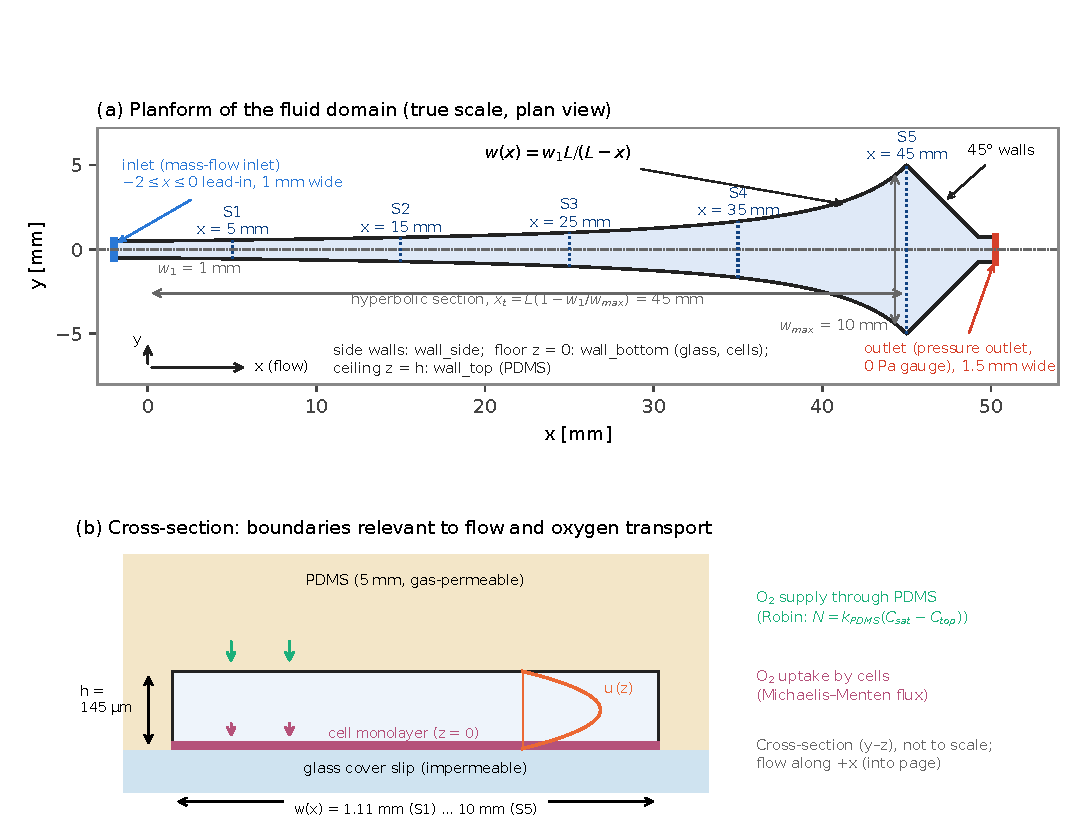
\includegraphics[width=0.92\linewidth]{geometry_schematic.pdf}
\caption{(a) Planform at true scale, with boundaries and stations S1--S5. (b) Cross-section (not to scale): cells on the glass floor, PDMS lid and side walls, and the oxygen fluxes used in \cref{sec:oxygen}.}
\label{fig:geometry}
\end{figure}

\subsection{Governing equations and regime}

The medium is incompressible and Newtonian ($\mu=\SI{0.94}{mPa.s}$, $\rho=\SI{981.8}{kg/m^3}$ at \SI{37}{\celsius} \citep{Delon2020}), and the flow is steady and laminar. The flow obeys
\begin{equation}
\nabla\cdot\bm u=0,\qquad \rho\,\bm u\cdot\nabla\bm u=-\nabla p+\mu\nabla^2\bm u,
\label{eq:ns}
\end{equation}
with no slip on all walls. Gravity is absorbed into the pressure, since there is no free surface. The Reynolds number on the hydraulic diameter at $x=0$ is $\Rey_{D_h}=0.0067$, 0.030 and 3.65 for the three flow rates. The relevant thin-gap measure is the ratio of convective to viscous forces, $\Rey_h\,h/\ell$, where $\ell=L-x$ is the length over which the width changes. It is bounded by $\Rey^*=\Rey_h\,h/w=\num{5.6e-4}$, \num{2.5e-3} and 0.30. Inertia is therefore negligible, and the flow should scale exactly with $Q$.

\subsection{Lubrication theory: three levels}
\label{sec:theory}

\paragraph{T1: parallel plates.} Relative to the dominant viscous term $\mu\,\partial^2u_x/\partial z^2$, axial diffusion is $O(h/\ell)^2\le10^{-4}$, transverse diffusion is $O(h/w)^2\le0.02$ (except within $\sim h$ of a side wall) and inertia is $O(\Rey^*)$. To leading order, \cref{eq:ns} reduces to $\partial p/\partial x=\mu\,\partial^2u_x/\partial z^2$ with $p=p(x,y)$. Integrating twice with $u_x(0)=u_x(h)=0$ gives
\begin{equation}
u_x=-\frac{1}{2\mu}\frac{\partial p}{\partial x}\,z(h-z),\qquad u_{\max}=-\frac{h^2}{8\mu}\frac{\partial p}{\partial x}.
\label{eq:parabola}
\end{equation}
The flux per unit width is $\bm q=-(h^3/12\mu)\nabla p$, and depth-integrated continuity gives $\nabla^2p=0$. If the iso-bars are straight across the width, $Q=w\,q_x$, and substituting \cref{eq:width} gives
\begin{equation}
\frac{\dd p}{\dd x}=-\frac{12\mu Q}{h^3w_1}\Big(1-\frac xL\Big),\qquad
p(0)-p(x)=\frac{12\mu Q}{h^3w_1}\Big(x-\frac{x^2}{2L}\Big),
\label{eq:dpdx}
\end{equation}
\begin{equation}
\taw=\mu\left.\frac{\partial u_x}{\partial z}\right|_{0}=\frac h2\left|\frac{\dd p}{\dd x}\right|=\frac{6\mu Q}{h^2w_1}\Big(1-\frac xL\Big)=\frac{4\mu u_{\max}}{h}.
\label{eq:eq2}
\end{equation}
\Cref{eq:eq2} is Eq.~2 of Delon \emph{et al.} The shear falls linearly by a factor $w_{\max}/w_1=10$, from \SI{0.0447}{\dyncm} at \SI{1}{\uLmin}. The identity $\taw=(h/2)|\dd p/\dd x|$ holds for any locally parabolic flow and is used below to check the CFD.

\paragraph{T2: side-wall correction.} For fully developed flow in a $w\times h$ rectangle, $\nabla^2_{yz}u_x=-G/\mu$ with $G=-\dd p/\dd x$. Write the solution as the parallel-plate profile plus a harmonic correction, and expand $z(h-z)$ in a sine series. This gives
\begin{gather}
u_x=\frac{G}{2\mu}\Big[z(h-z)-\sum_{n\ \mathrm{odd}}\frac{8h^2}{\pi^3n^3}\sin\frac{n\pi z}{h}\,\frac{\cosh(n\pi y/h)}{\cosh(n\pi w/2h)}\Big],
\label{eq:rect}\\
f\Big(\frac hw\Big)=1-\frac{192h}{\pi^5w}\sum_{n\ \mathrm{odd}}\frac{\tanh(n\pi w/2h)}{n^5}\approx1-0.63\frac hw ,
\label{eq:flux}
\end{gather}
where $Q=Gwh^3f/12\mu$. At a given $Q$, the gradient and the axial floor shear rise by $1/f$, i.e.\ by 9.0, 6.8, 4.8, 2.8 and \SI{0.9}{\percent} at S1--S5. Differentiating \cref{eq:rect} at $z=0$, the floor shear near a side wall is $\tau/\tau(0)\approx1-(8/\pi^2)e^{-\pi\delta/h}$, where $\delta$ is the distance from the wall. It is therefore more than a fraction $\varepsilon$ below the core value within
\begin{equation}
\delta_\varepsilon=\frac h\pi\ln\frac{8}{\pi^2\varepsilon}=\SI{0.129}{mm}\quad(\varepsilon=\SI{5}{\percent}),
\label{eq:delta}
\end{equation}
independently of $w$. The half-width of uniform shear is $d=w/2-\delta_\varepsilon$.

\paragraph{T3: two-dimensional planform model.} Near the outlet corner the iso-bars curve and \cref{eq:dpdx} fails. To capture this, we solved $\nabla\cdot[K\nabla p]=0$, with $K=h^3f(h/w)/12\mu$, on the complete planform with linear finite elements (\SI{20}{\micro\metre} axial spacing). The boundary conditions are zero normal flux on the side walls, a uniform inflow at the inlet and $p=0$ at the outlet. The axial shear is $(h/2)|\nabla p|$. T3 reduces to T2 where the planform varies slowly. It predicts a shear minimum at $x=\SI{44.1}{mm}$ and a value at S5 that is \SI{54}{\percent} above \cref{eq:eq2} (\cref{fig:T3}).

\begin{figure}[t]
\centering
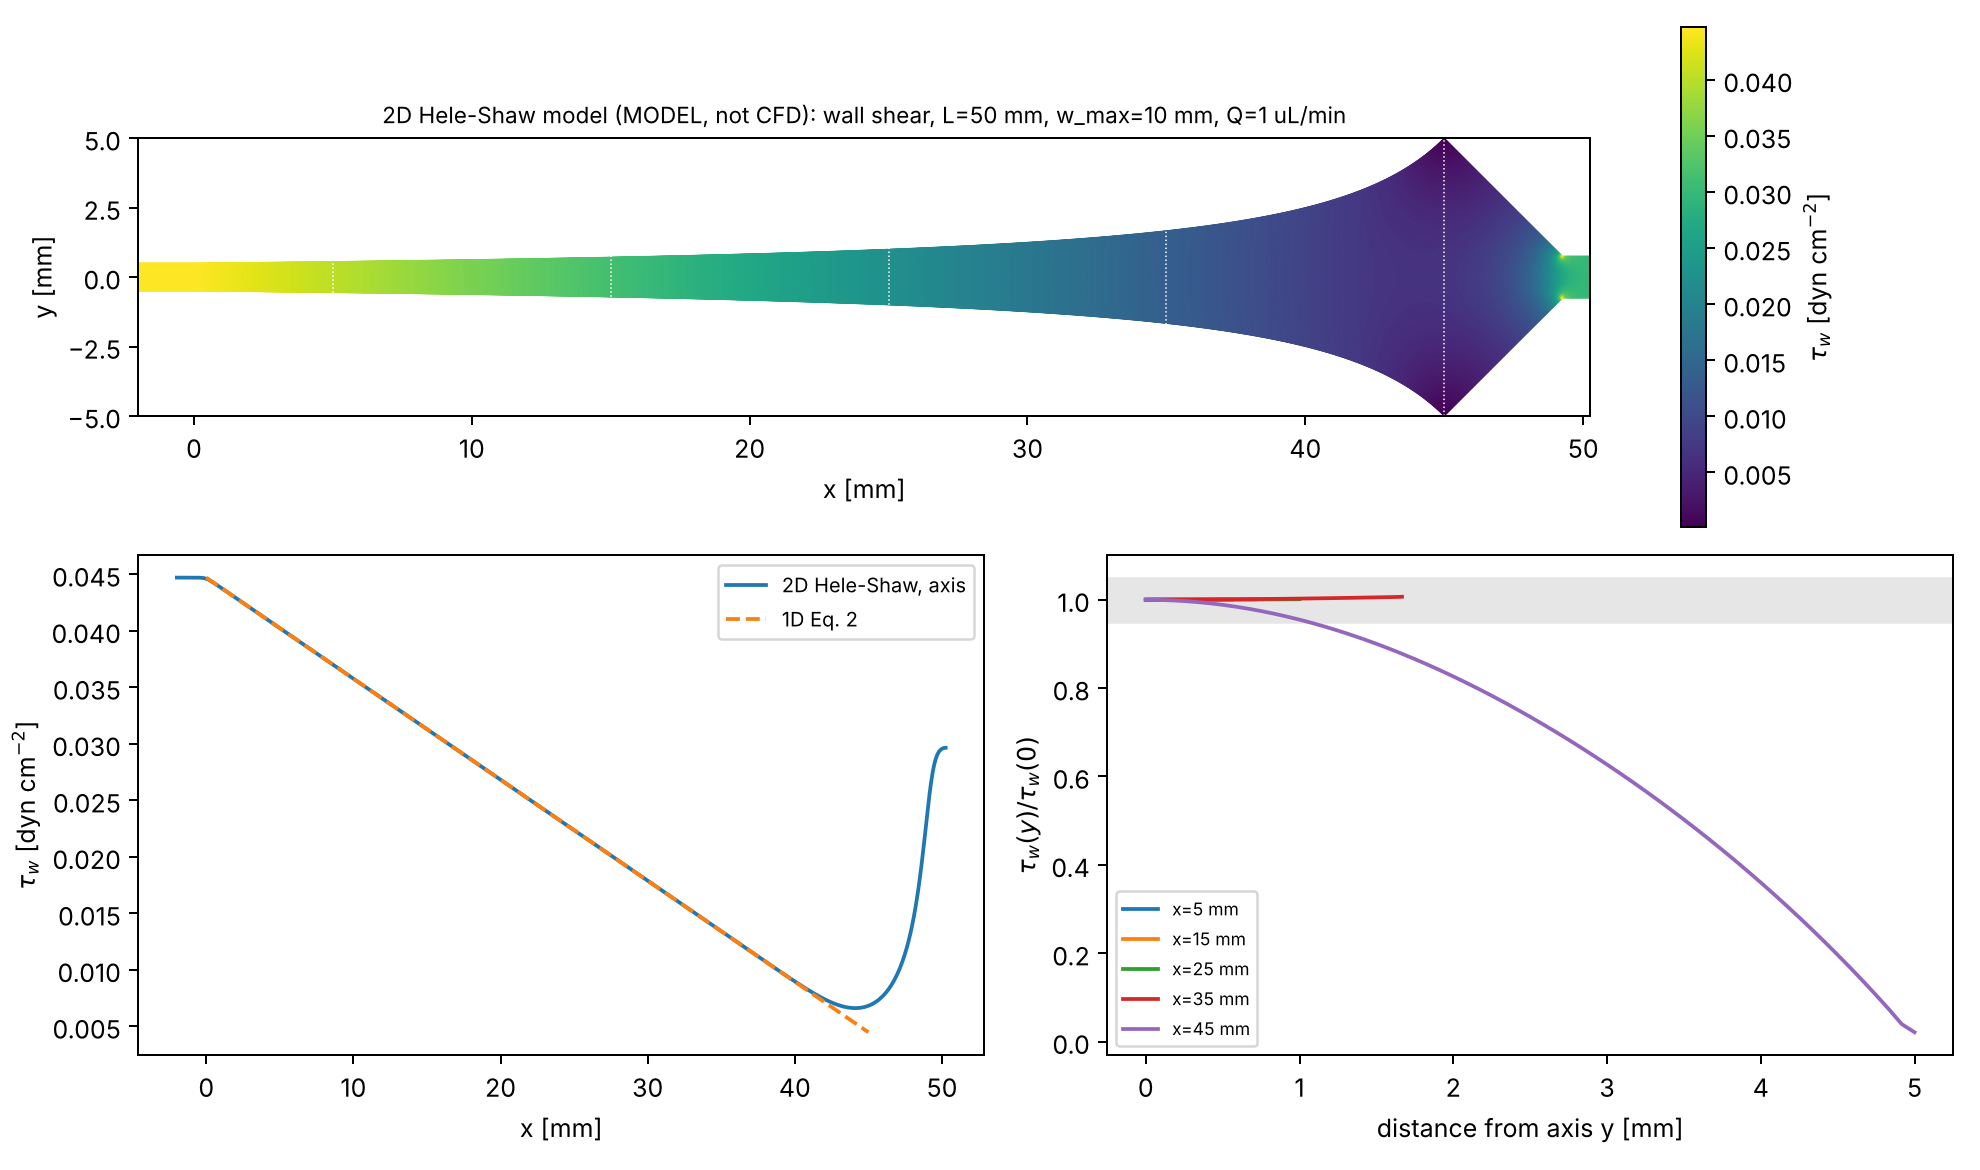
\includegraphics[width=0.82\linewidth]{T3_hs2d_W10_Q1.png}
\caption{Model T3 at \SI{1}{\uLmin}. Top: floor shear over the planform. Bottom left: axial shear against Eq.~2; the two separate beyond $x\approx\SI{40}{mm}$ because of the outlet corner. Bottom right: transverse profiles, flat at S1--S4 (T3 has no side-wall layer) and dome-shaped at S5.}
\label{fig:T3}
\end{figure}

\subsection{Numerical method}

The geometry was built as a STEP solid (CadQuery) and simulated in ANSYS Fluent 2024 R1 with the settings in \cref{tab:setup}. The mesh was not documented in the results we received. The exported cross-section nodes show four distinct interior velocity levels, each appearing twice, which implies about nine cell layers across the gap. The wall nodes are \SIrange{0.08}{0.10}{mm} apart near the side walls. Initial runs with absolute residual criteria of $10^{-6}$ reported convergence after three iterations. This is meaningless at mass flows of order \SI{e-9}{kg/s}, so the criterion was replaced by monitoring the solution. The exports contain no residual history or mass balance, so convergence was judged from internal consistency (\cref{sec:validation}). Only one mesh was run. A grid-convergence study (GCI \citep{Roache1994,Celik2008}) with $N_z=9$, 18 and 36 layers and in-plane sizes of 100, 50 and \SI{25}{\micro\metre} has been designed but not yet performed.

\begin{table}[t]
\centering
\caption{Simulation set-up (present work) compared with the reference CFD \citep{Delon2020}.}
\label{tab:setup}
\small
\begin{tabularx}{\linewidth}{@{}p{0.2\linewidth}XX@{}}
\toprule
 & Delon \emph{et al.} (2020) & Present\\
\midrule
Domain & 3D chamber with ports; $h=\SI{150}{\micro\metre}$ (CFD) & 3D planar domain, lead-in and outlet duct; $h=\SI{145}{\micro\metre}$\\
Flow rates & 0.22, 1 (120 in supplement) \ulmin & $\dot m=\num{3.6e-9}$, \num{1.636e-8}, \SI{1.964e-6}{kg/s} (0.2200, 0.9998, \SI{120.02}{\uLmin})\\
Boundary conditions & uniform mass-flow inlet, atmospheric outlet, no slip & mass-flow inlet, \SI{0}{Pa} gauge pressure outlet, no slip\\
Solver & transient ($\Delta t=\SI{e-7}{s}$), SIMPLE, PRESTO!, 2nd-order upwind & steady, laminar, double precision, SIMPLEC, PRESTO!, 2nd-order upwind; URF 0.3/0.7\\
Mesh & tetrahedral, ``max.\ \SI{5}{\micro\metre}'', \SI{1.4}{\percent} sensitivity & $\approx9$ layers across $h$ (inferred); one mesh\\
\bottomrule
\end{tabularx}
\end{table}

% =====================================================================
\section{Flow results and validation}
\label{sec:validation}

\subsection{Comparison with the published results}

The paper gives its results only as plots and ranges, and the curves were not digitised, so \cref{tab:published} compares the values it states explicitly. The shear range is reproduced at both flow rates. Both studies find the downstream minimum above the end value of \cref{eq:eq2}, which is the outlet-corner effect predicted by T3. The paper's equation range for \SI{1}{\uLmin} (lower bound 0.008) corresponds to evaluating \cref{eq:eq2} with $L=\SI{5.3}{cm}$ at $x\approx\SI{5}{cm}$ (our inference). This explains the factor-of-two gap between its equation and CFD lower bounds.

The imaging half-widths agree with the published $D_{\max}$ to within \SI{2}{\percent} at S3--S4 and are 15--\SI{17}{\percent} wider at S1--S2 (\cref{fig:published}). The paper's criterion is not stated, and our values at the stricter $\pm\SI{2}{\percent}$ tolerance bracket its numbers. At S5 the published \SI{3.84}{mm} disagrees with our \SI{1.02}{mm}. T3 independently gives \SI{1.05}{mm}, and the published $D_{\mathrm{wall}}+D_{\max}$ does not equal the half-width at S5, which suggests a different planform there.

\begin{table}[t]
\centering
\caption{Values stated by Delon \emph{et al.}~\citep{Delon2020} compared with the present CFD and with \cref{eq:eq2} for $L=\SI{50}{mm}$. Shear in \si{\dyncm}; $\tau_{\mathrm{cell}}=3\taw$ as in the paper.}
\label{tab:published}
\small
\begin{tabular}{@{}llccc@{}}
\toprule
Quantity & $Q$ [\ulmin] & Published & Present CFD & \cref{eq:eq2}\\
\midrule
$\taw$ at inlet & 0.22 & $\sim$0.01 & 0.0102 & 0.0098\\
$\taw$ downstream minimum & 0.22 & $\sim$0.001 & 0.0014 ($x=\SI{44}{mm}$) & 0.0010 ($x=\SI{45}{mm}$)\\
$\taw$ at inlet & 1 & 0.0447 & 0.0464 & 0.0447\\
$\taw$ downstream minimum & 1 & 0.0059 & 0.0063 ($x=\SI{44}{mm}$) & 0.0045 ($x=\SI{45}{mm}$)\\
$\tau_{\mathrm{cell}}$ range (CFD) & 1 & $\sim$0.134--0.017 & 0.139--0.019 & --\\
Uniform zone independent of $Q$ & all & yes & yes ($<\SI{0.002}{mm}$) & --\\
\bottomrule
\end{tabular}
\end{table}

\begin{figure}[t]
\centering
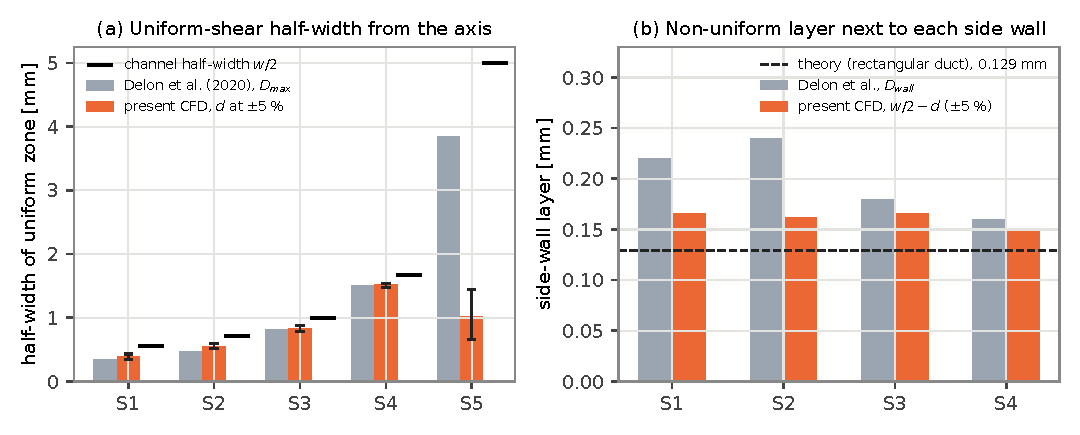
\includegraphics[width=0.9\linewidth]{published_vs_present_uniform_zone.pdf}
\caption{Imaging zone: Delon \emph{et al.}\ (Table~2 of \citep{Delon2020}) against the present CFD at \SI{1}{\uLmin}. (a) Half-width of the uniform-shear band; error bars span $\pm2$ to $\pm\SI{10}{\percent}$ tolerance. (b) Non-uniform layer at each side wall, with \cref{eq:delta}.}
\label{fig:published}
\end{figure}

\subsection{Pressure and wall shear along the axis}

\Cref{fig:contours} shows the Fluent fields. The iso-bars are straight across the narrow part, as \cref{eq:dpdx} assumes, and bend only near the outlet corner. The wall-shear colour scale is dominated by a local peak at the inlet face of the lead-in, caused by the uniform inlet velocity. This peak decays within \SI{0.1}{mm} and does not affect the hyperbolic section.

\begin{figure}[t]
\centering
\begin{subfigure}[t]{0.44\linewidth}\centering
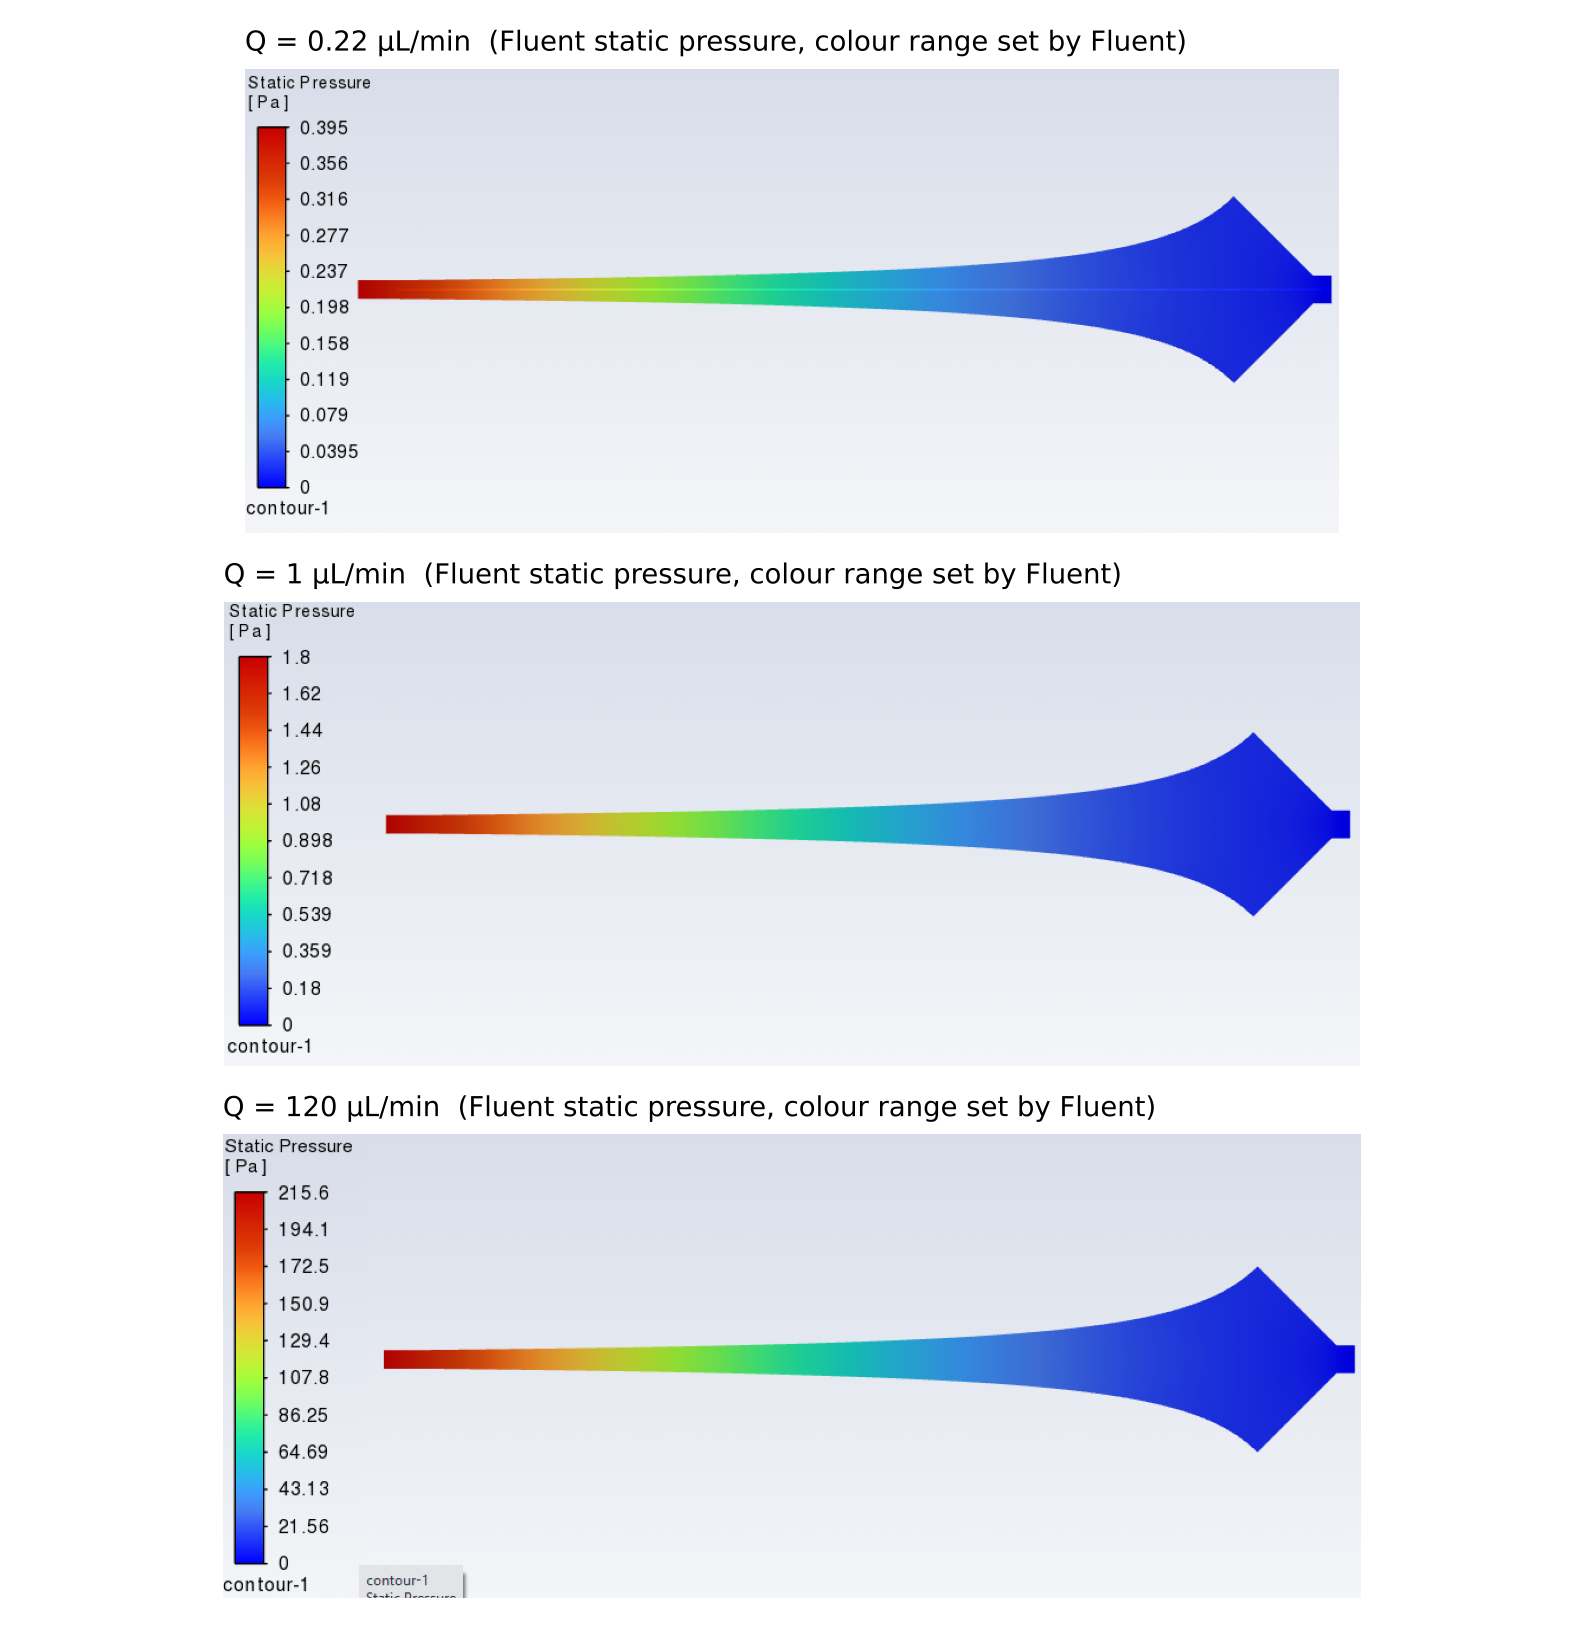
\includegraphics[width=\linewidth]{Fig01_pressure_contours_all_Q.png}
\caption{Static pressure.}
\end{subfigure}\hspace{4mm}
\begin{subfigure}[t]{0.44\linewidth}\centering
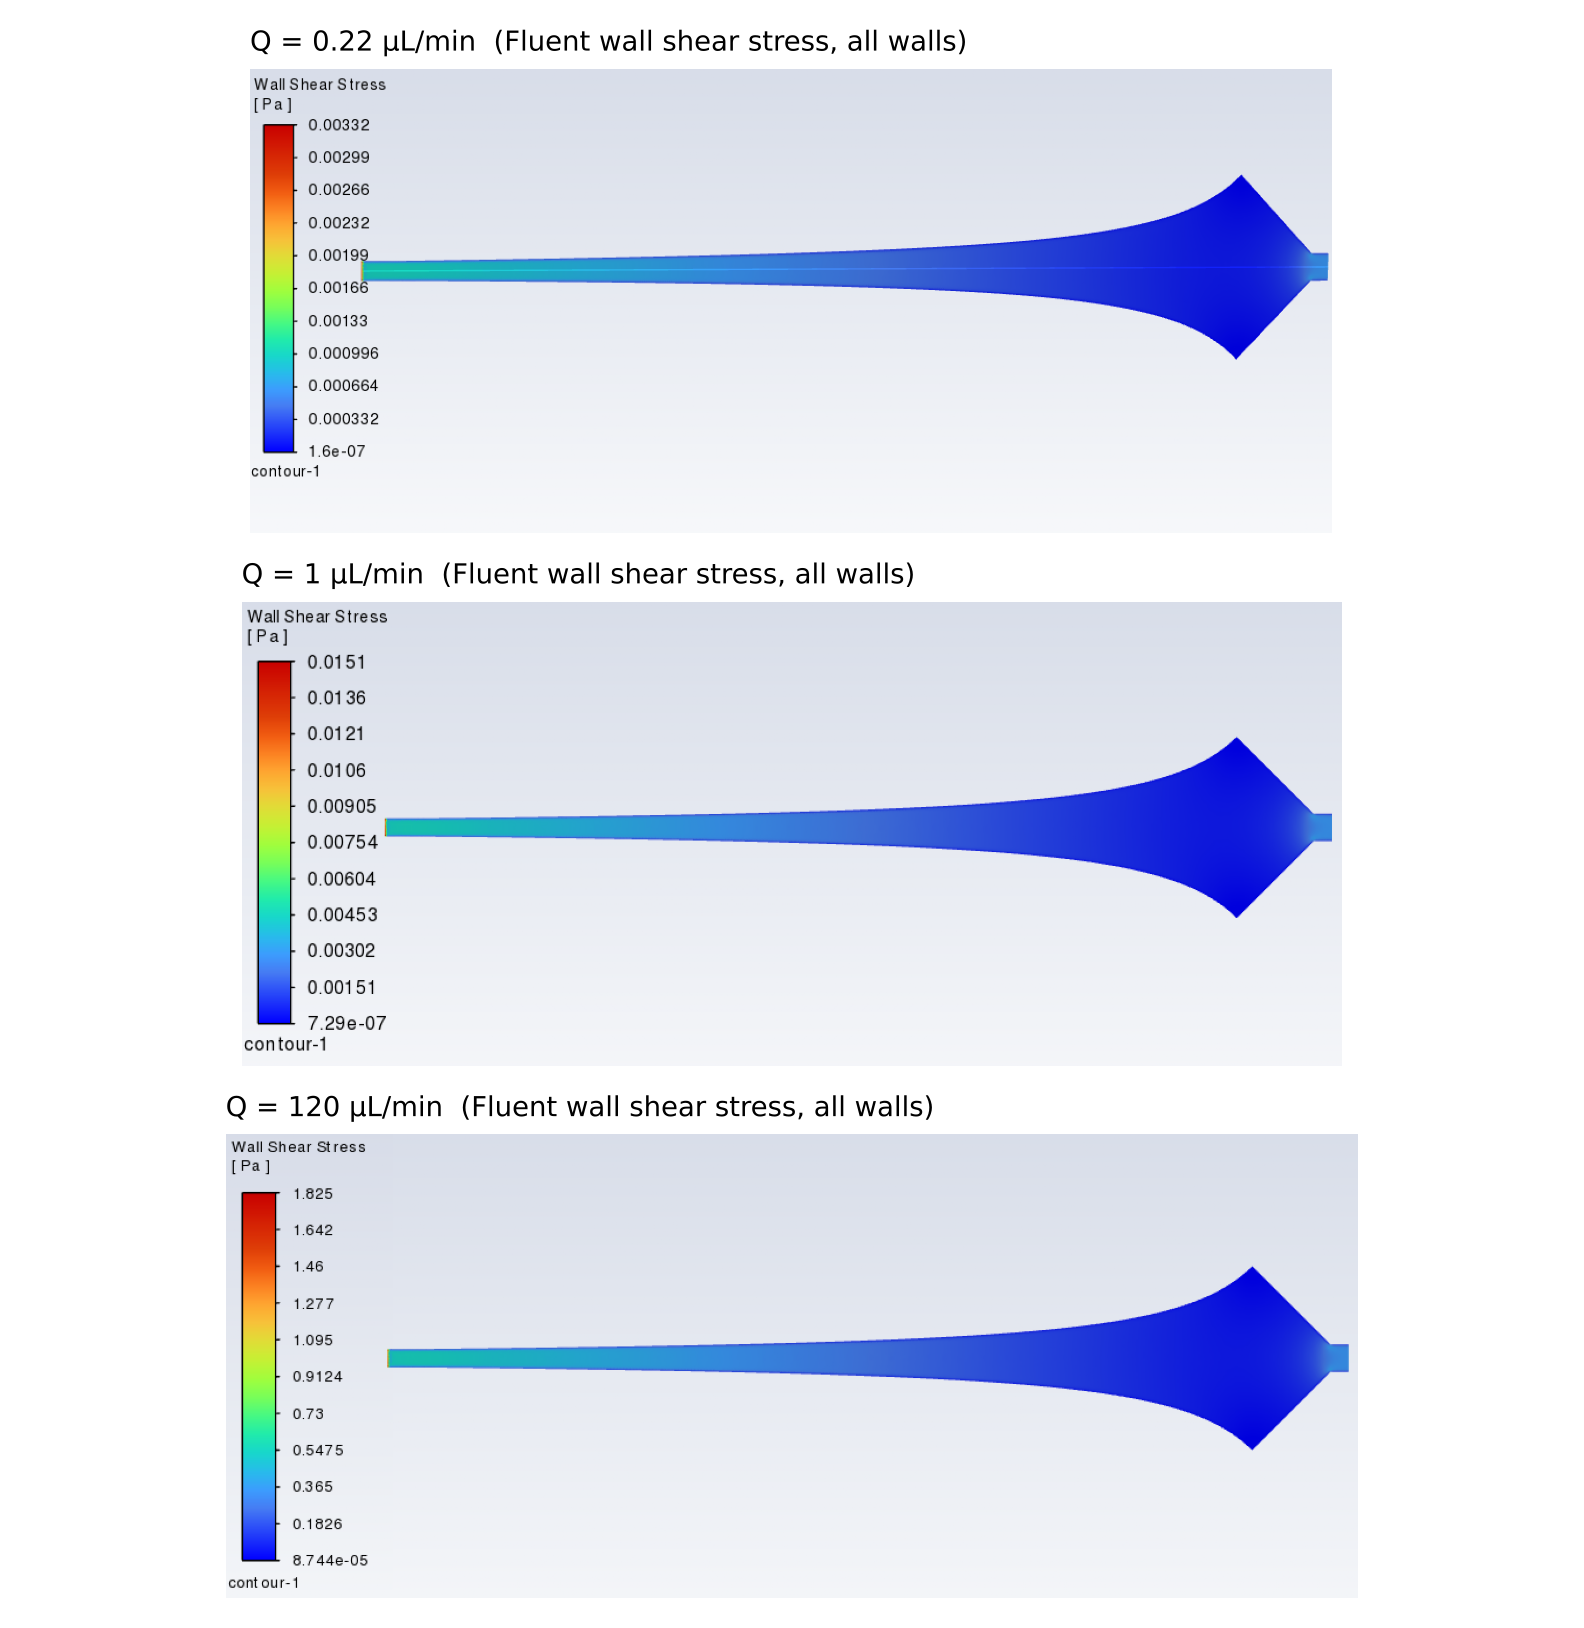
\includegraphics[width=\linewidth]{Fig09_wall_shear_contours_all_Q.png}
\caption{Wall shear stress.}
\end{subfigure}
\caption{Fluent contours at 0.22 (top), 1 (middle) and \SI{120}{\uLmin} (bottom). The colour-bar maxima scale with $Q$ to within \SI{0.3}{\percent} (pressure) and \SI{0.7}{\percent} (shear).}
\label{fig:contours}
\end{figure}

The axial pressure decreases monotonically at all 730 exported positions. Its profile, normalised by $p(0)$, follows T3 to within \SI{0.08}{\percent} of $p(0)$, including the gradient minimum at $x\approx\SI{44}{mm}$ and the steep fall through the outlet. The drop from $x=0$ to the outlet is $\Delta p=1.657\,Q$ (Pa, $Q$ in \ulmin; $R^2=1.000000$), so the hydraulic resistance is \SI{9.94e10}{Pa.s/m^3} at all three flow rates (\cref{fig:pressure}). Over the hyperbolic section the CFD drop is \SI{1.4}{\percent} above T1 and \SI{4.9}{\percent} below T2. The local gradient falls from 63 to a minimum of \SI{8.7}{Pa/m} per \ulmin\ at $x=\SI{43.9}{mm}$, a factor of 7.3 rather than the factor of 10 of \cref{eq:dpdx}, because the flow already begins to converge towards the outlet. T3 places the minimum at \SI{44.1}{mm}.

\begin{figure}[t]
\centering
\begin{subfigure}[t]{0.49\linewidth}\centering
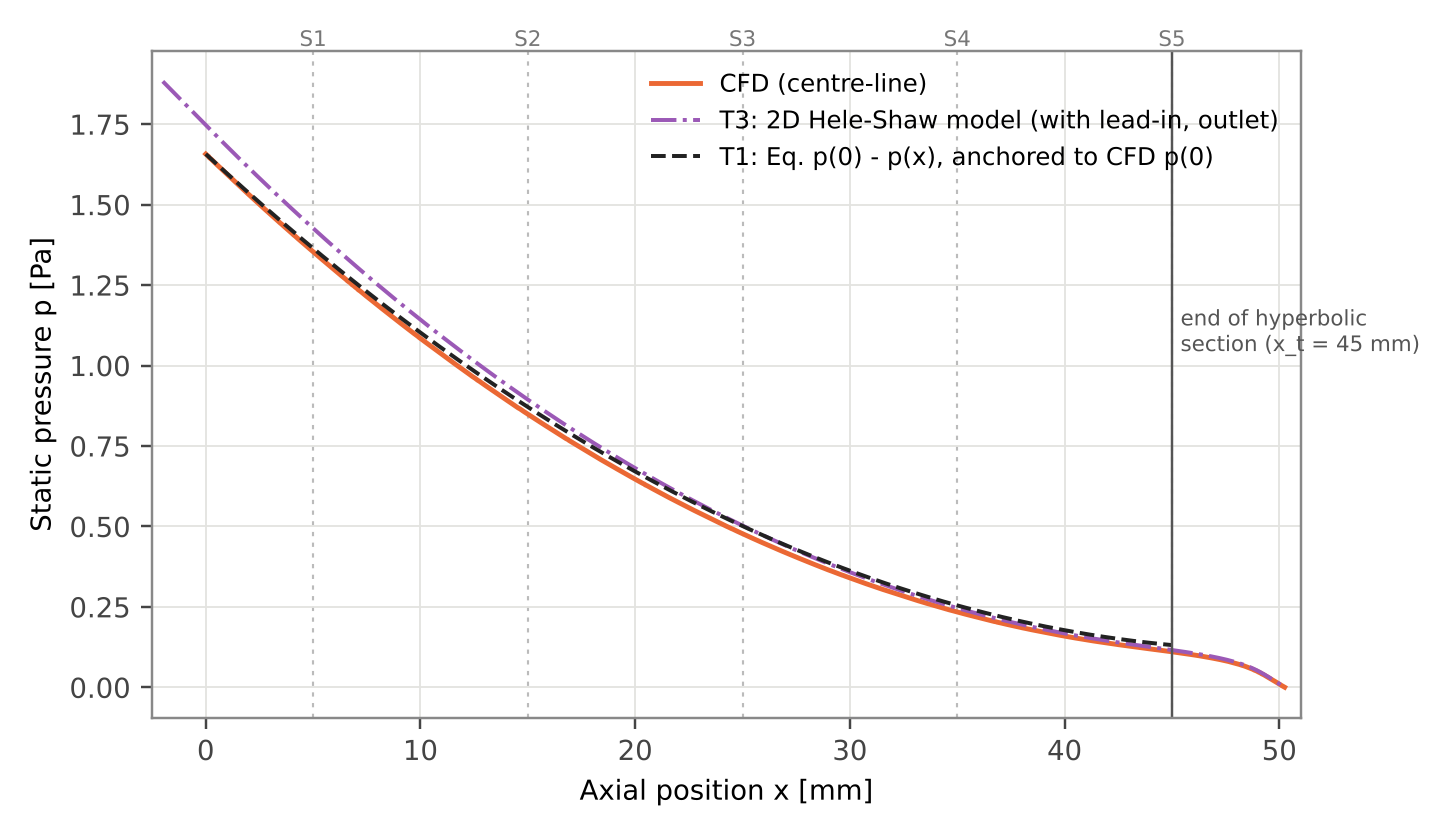
\includegraphics[width=\linewidth]{Fig03_pressure_vs_x_Q1.png}
\caption{Axial pressure at \SI{1}{\uLmin}.}
\end{subfigure}\hfill
\begin{subfigure}[t]{0.49\linewidth}\centering
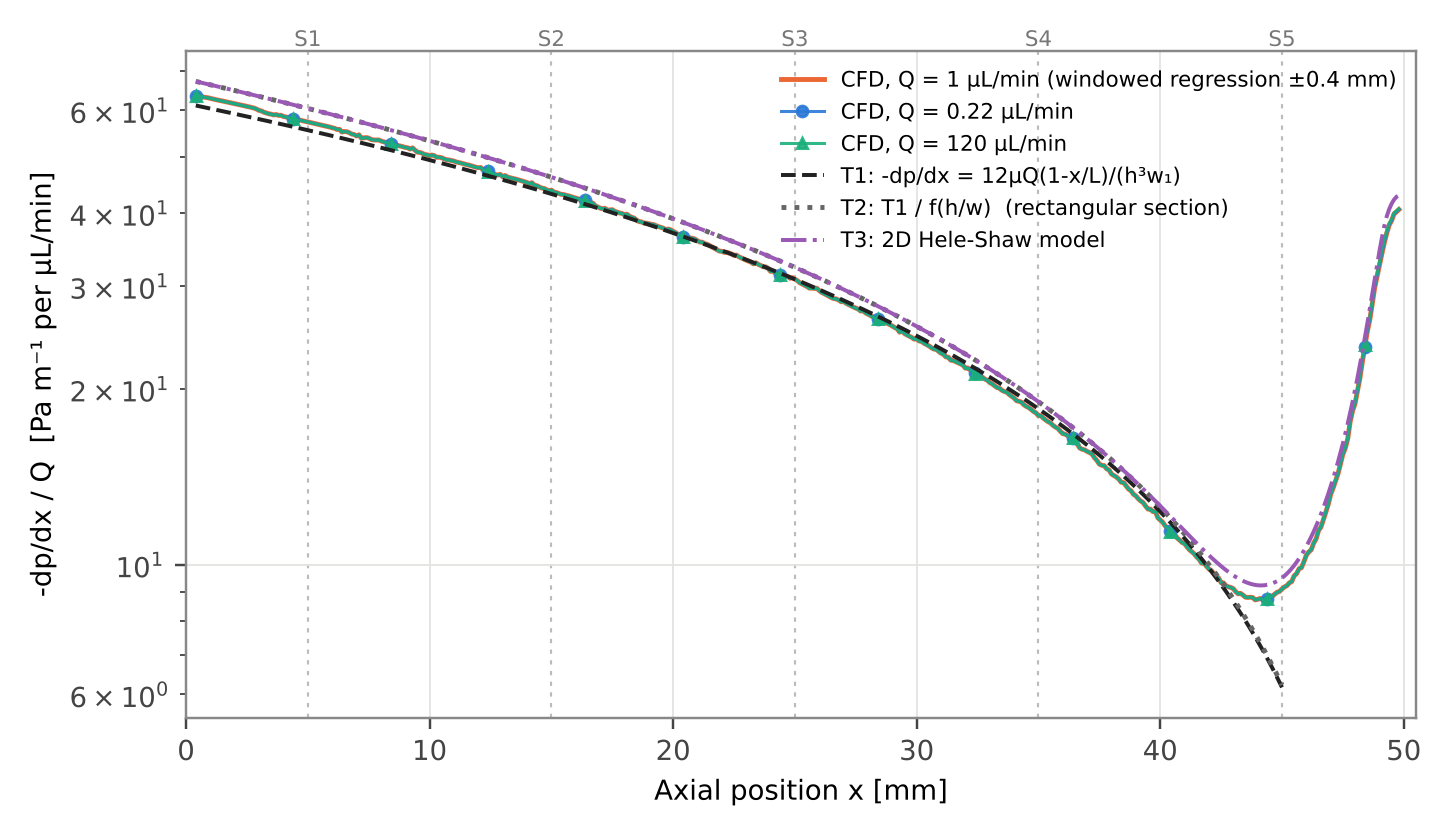
\includegraphics[width=\linewidth]{Fig07_pressure_gradient_vs_x.png}
\caption{Local pressure gradient per unit $Q$.}
\end{subfigure}
\caption{(a) CFD pressure against T3 (absolute) and T1 (anchored at $x=0$). (b) $|\dd p/\dd x|/Q$ from a $\pm\SI{0.4}{mm}$ least-squares window. It falls linearly, reaches a minimum near \SI{44}{mm}, and rises in the converging outlet.}
\label{fig:pressure}
\end{figure}

\Cref{fig:tau} and \cref{tab:stations} compare the axial wall shear with theory. Over 2--\SI{40}{mm} the RMSE relative to the mean is \SI{2.5}{\percent} against T1 and \SI{5.6}{\percent} against T2 and T3. Taken alone, this would favour Eq.~2. The structure of the deviation shows otherwise (\cref{fig:tau}b). Plotted against $h/w$, the deviation from T1 runs parallel to the exact side-wall correction $1/f-1$: the residual slope is $-0.026$ per unit $h/w$, with a scatter of $\pm\SI{0.36}{\percent}$, and the line is shifted down by \SI{4.9}{\percent}. The CFD thus captures the side-wall drag that Eq.~2 omits, with the correct coefficient, and carries an additional uniform offset. Near the inlet the two effects partly cancel (\SI{+9}{\percent} and \SI{-5}{\percent}), and at S3 they cancel exactly. A straight line fitted to the CFD reaches zero at $x=\SI{48.8}{mm}$, not at $L$. T2 gives the same value, so the curvature is physical.

At S5 the shear is \SI{46.5}{\percent} above Eq.~2, but only \SI{4.9}{\percent} below T3 (\cref{fig:deviation}a). Ratios that cancel any uniform offset, $\taw(\mathrm{S}k)/\taw(\mathrm{S}3)=1.862$, 1.413, 0.589 and 0.294, agree with T3 to within \SI{1}{\percent} at every station, S5 included. Eq.~2 errs in these ratios by $+3.5$ to \SI{+47}{\percent}. The CFD field is, to a good approximation, the T3 field multiplied by 0.95 ($p_{\mathrm{CFD}}/p_{T3}=0.950\pm0.001$ along 0--\SI{49.5}{mm}).

\begin{figure}[t]
\centering
\begin{subfigure}[t]{0.49\linewidth}\centering
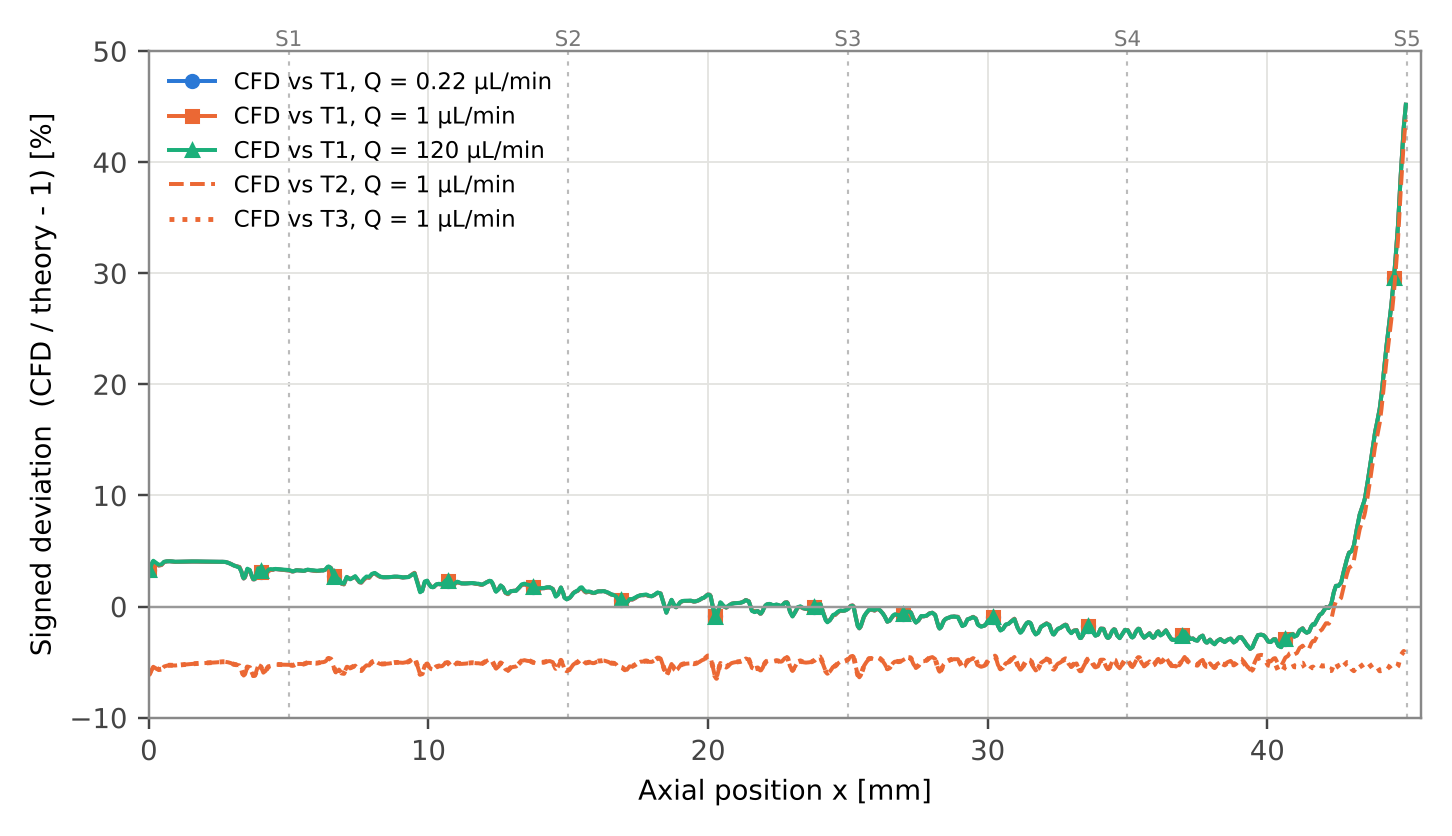
\includegraphics[width=\linewidth]{Fig15_wall_shear_percentage_deviation.png}
\caption{Signed deviation along $x$.}
\end{subfigure}\hfill
\begin{subfigure}[t]{0.49\linewidth}\centering
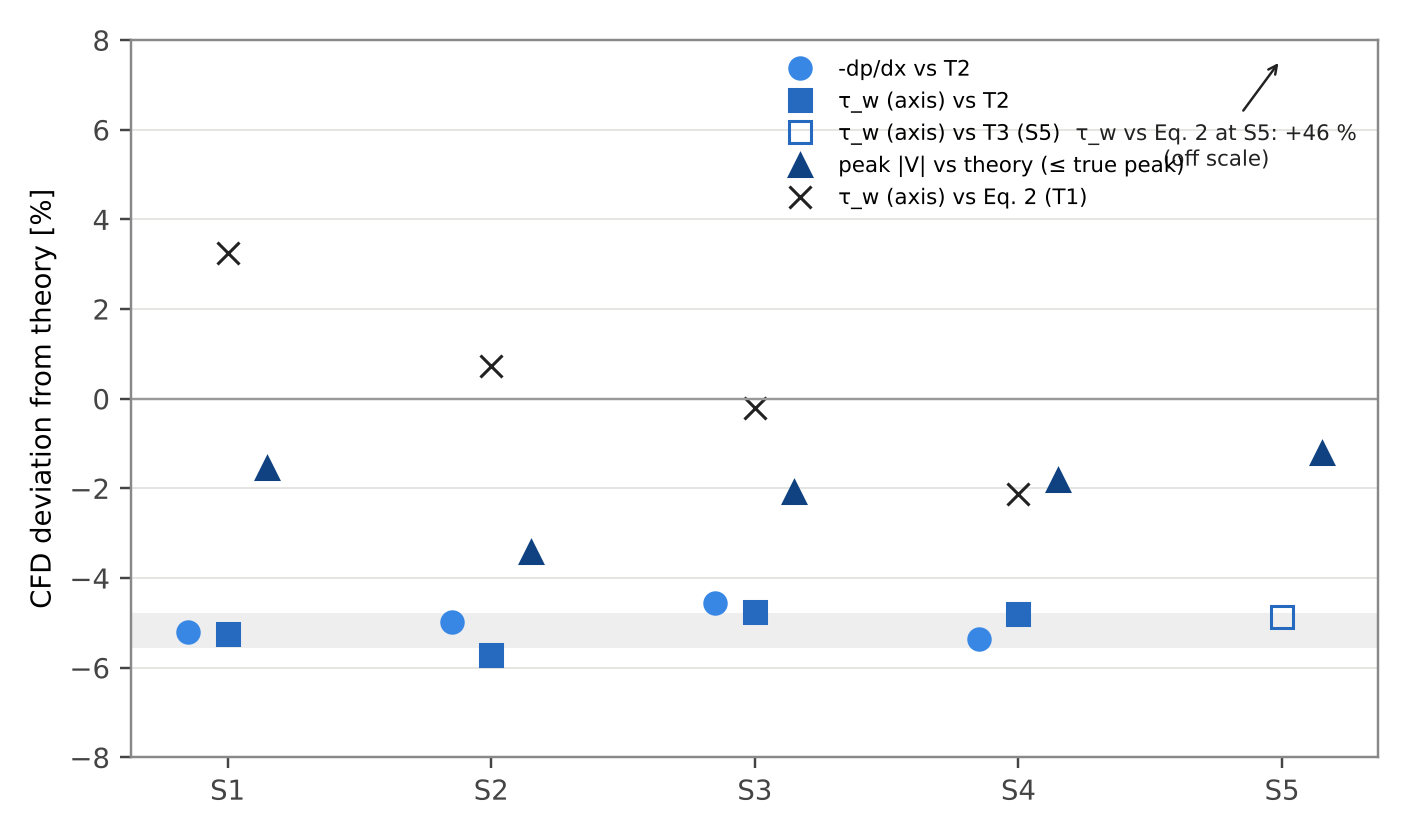
\includegraphics[width=\linewidth]{Fig37_validation_ratios_by_station.png}
\caption{Deviation from the best applicable theory.}
\end{subfigure}
\caption{(a) Deviation of the CFD axial shear from T1, T2 and T3. Against T1 it changes sign near \SI{23}{mm} and jumps to \SI{+46}{\percent} at S5; against T2/T3 it is a near-constant \SI{-5}{\percent}. (b) Pressure gradient, shear and peak velocity relative to T2 (S1--S4) or T3 (S5); crosses mark Eq.~2. The grey band is the mean $\pm$ s.d.\ over 2--\SI{40}{mm}.}
\label{fig:deviation}
\end{figure}

\begin{figure}[t]
\centering
\begin{subfigure}[t]{0.5\linewidth}\centering
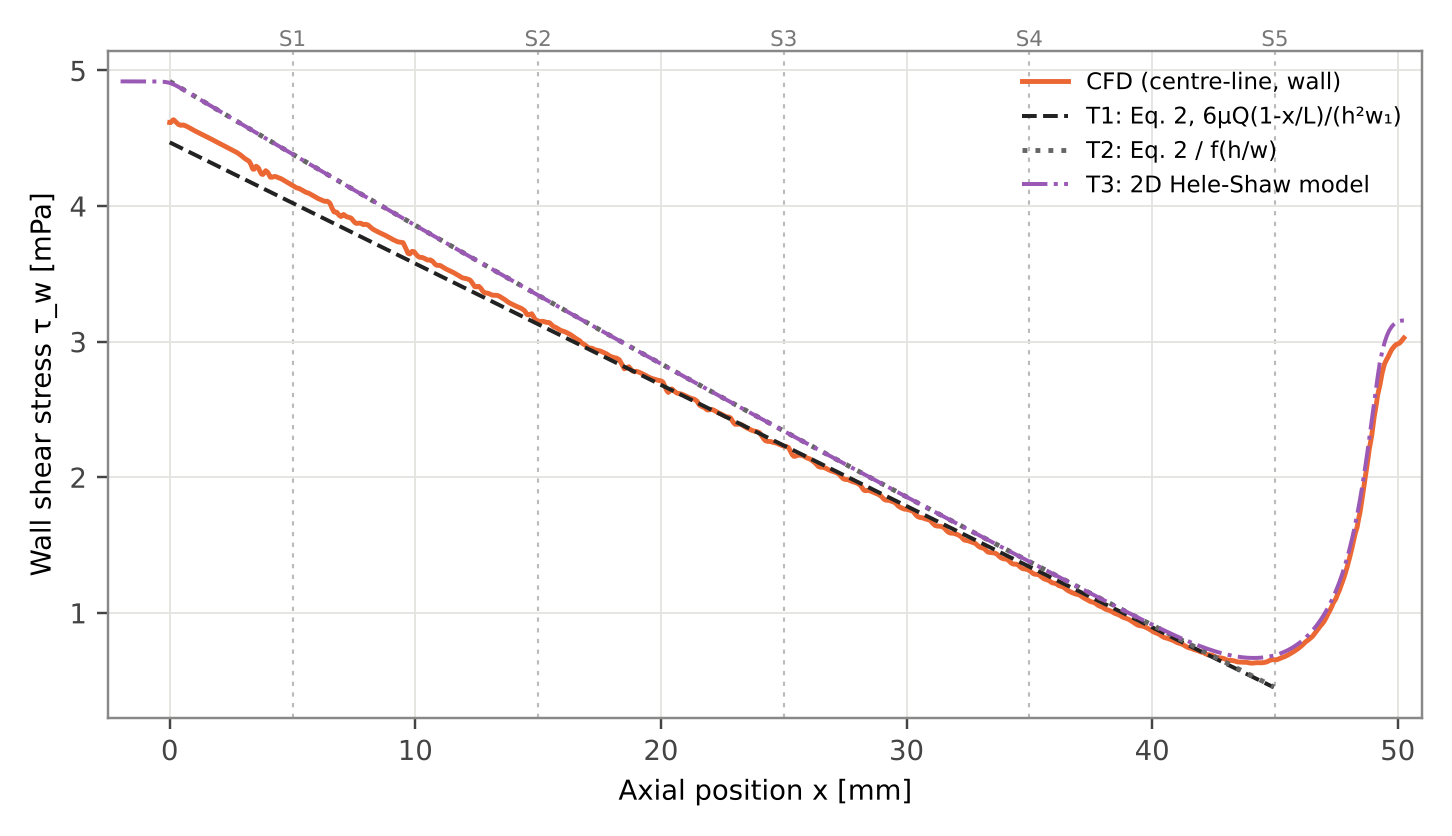
\includegraphics[width=\linewidth]{Fig11_wall_shear_vs_x_Q1.png}
\caption{Axial wall shear at \SI{1}{\uLmin}.}
\end{subfigure}\hfill
\begin{subfigure}[t]{0.48\linewidth}\centering
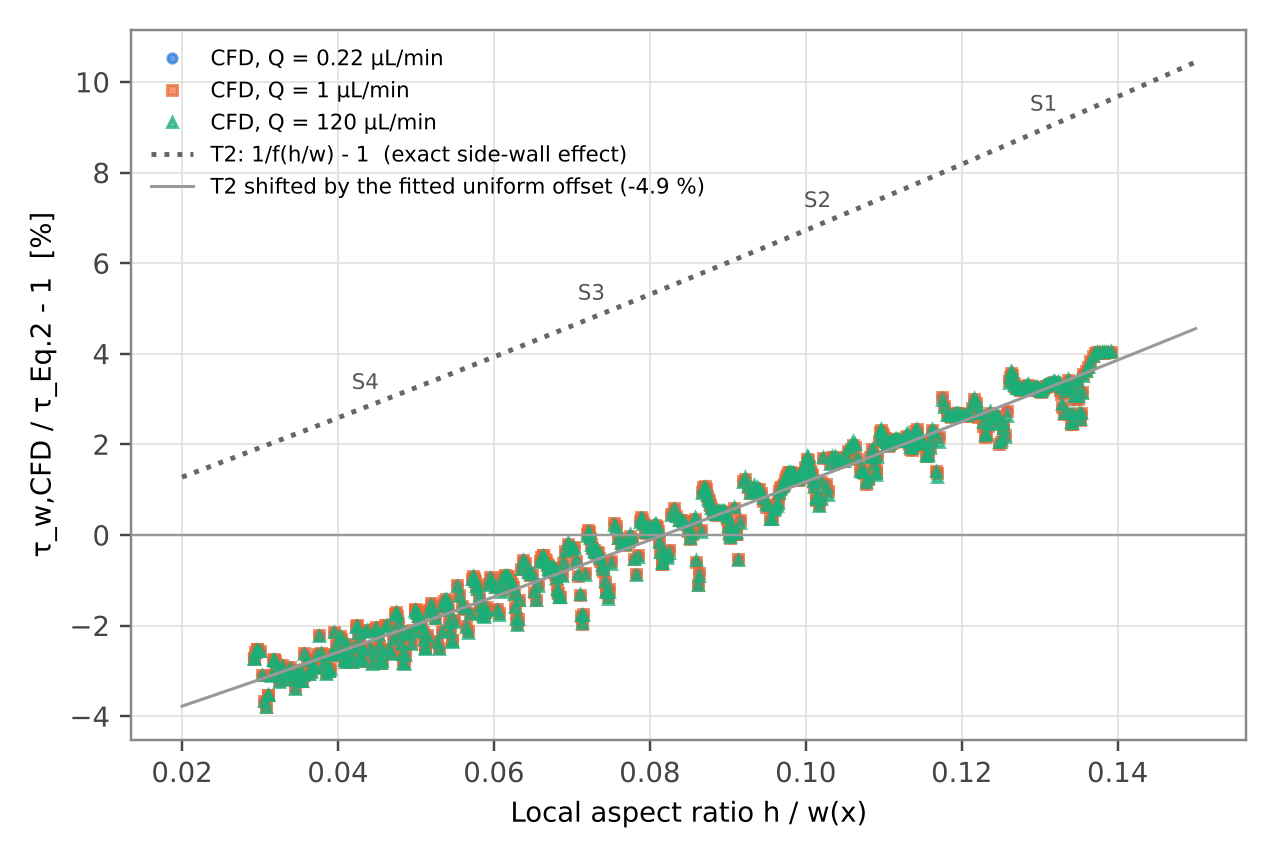
\includegraphics[width=\linewidth]{Fig16_shear_deviation_vs_aspect_ratio.png}
\caption{Deviation from Eq.~2 against $h/w$.}
\end{subfigure}
\caption{(a) CFD against T1 (Eq.~2), T2 and T3. The CFD runs parallel to T2/T3 about \SI{5}{\percent} lower, crosses T1 near $x=\SI{23}{mm}$, and follows T3 through the minimum at \SI{44}{mm} and the rise in the outlet. (b) CFD points ($2\le x\le\SI{40}{mm}$) lie on a line parallel to the side-wall correction $1/f-1$, shifted by \SI{-4.9}{\percent}.}
\label{fig:tau}
\end{figure}

\begin{table}[t]
\centering
\caption{Axial wall shear at \SI{1}{\uLmin}; the other flow rates give identical relative deviations to within \SI{0.04}{\percent}. Momentum balance: CFD $\taw$ divided by $(h/2)|\dd p/\dd x|$ computed from the CFD pressure.}
\label{tab:stations}
\small
\begin{tabular}{@{}lcccccc@{}}
\toprule
Station & $h/w$ & $\taw$ CFD [mPa] & vs T1 [\%] & vs T2 [\%] & vs T3 [\%] & Momentum balance\\
\midrule
S1 & 0.131 & 4.154 & $+3.25$ & $-5.24$ & $-5.23$ & 0.9995\\
S2 & 0.102 & 3.152 & $+0.72$ & $-5.72$ & $-5.71$ & 0.9922\\
S3 & 0.073 & 2.230 & $-0.21$ & $-4.77$ & $-4.75$ & 0.9978\\
S4 & 0.044 & 1.313 & $-2.12$ & $-4.81$ & $-4.79$ & 1.0057\\
S5 & 0.015 & 0.655 & $+46.47$ & n/a & $-4.87$ & 0.9936\\
\bottomrule
\end{tabular}
\end{table}

\subsection{Transverse distribution and imaging zone}

At S1--S4 the floor shear forms a flat plateau, varying by 0.1--\SI{0.7}{\percent} over the central half of the width. It falls near each side wall within a layer whose thickness is the same at every station (\cref{fig:transverse}). Plotted against the distance from the wall, the four profiles collapse onto one curve, as \cref{eq:delta} predicts. The measured layer is \SIrange{0.149}{0.166}{mm} thick against \SI{0.129}{mm} from theory. The difference is below the spacing of the wall nodes, so it is not resolved. Because the layer has a fixed thickness while the channel widens, the fraction of the width with uniform shear ($\pm\SI{5}{\percent}$) grows from \SI{70}{\percent} at S1 to 77, 83 and \SI{91}{\percent} at S2--S4. At S5, which is the corner, the profile is a dome and only \SI{20}{\percent} of the width is uniform (T3: \SI{21}{\percent}). These widths differ by less than \SI{0.002}{mm} between 0.22 and \SI{120}{\uLmin} (\cref{tab:uniform}). At S4 the result is insensitive to the tolerance, but at S5, which has no plateau, it changes by $-35$ to \SI{+42}{\percent}.

\begin{table}[t]
\centering
\caption{Uniform-shear zone at \SI{1}{\uLmin}. $d$ is the half-width within $\pm\varepsilon$ of the axis value. Theory: T2 at S1--S4 and T3 at S5.}
\label{tab:uniform}
\small
\begin{tabular}{@{}lcccccc@{}}
\toprule
Station & $w/2$ [mm] & $d$ ($\pm5\,\%$) [mm] & $d$ theory [mm] & side layer [mm] & $2d/w$ at $\pm2/5/10\,\%$ & Delon $D_{\max}$ [mm]\\
\midrule
S1 & 0.556 & 0.390 & 0.427 & 0.165 & 63 / 70 / 77 & 0.34\\
S2 & 0.714 & 0.552 & 0.586 & 0.162 & 72 / 77 / 83 & 0.47\\
S3 & 1.000 & 0.834 & 0.871 & 0.166 & 79 / 83 / 87 & 0.82\\
S4 & 1.667 & 1.518 & 1.538 & 0.149 & 88 / 91 / 92 & 1.5\\
S5 & 5.000 & 1.024 & 1.050 & -- & 13 / 20 / 29 & 3.84\\
\bottomrule
\end{tabular}
\end{table} Cells should therefore be imaged in the centre of S2--S4, at least \SI{0.17}{mm} from the side walls. Shear values for S5 must come from CFD or T3, not from Eq.~2.

\begin{figure}[t]
\centering
\begin{subfigure}[t]{0.49\linewidth}\centering
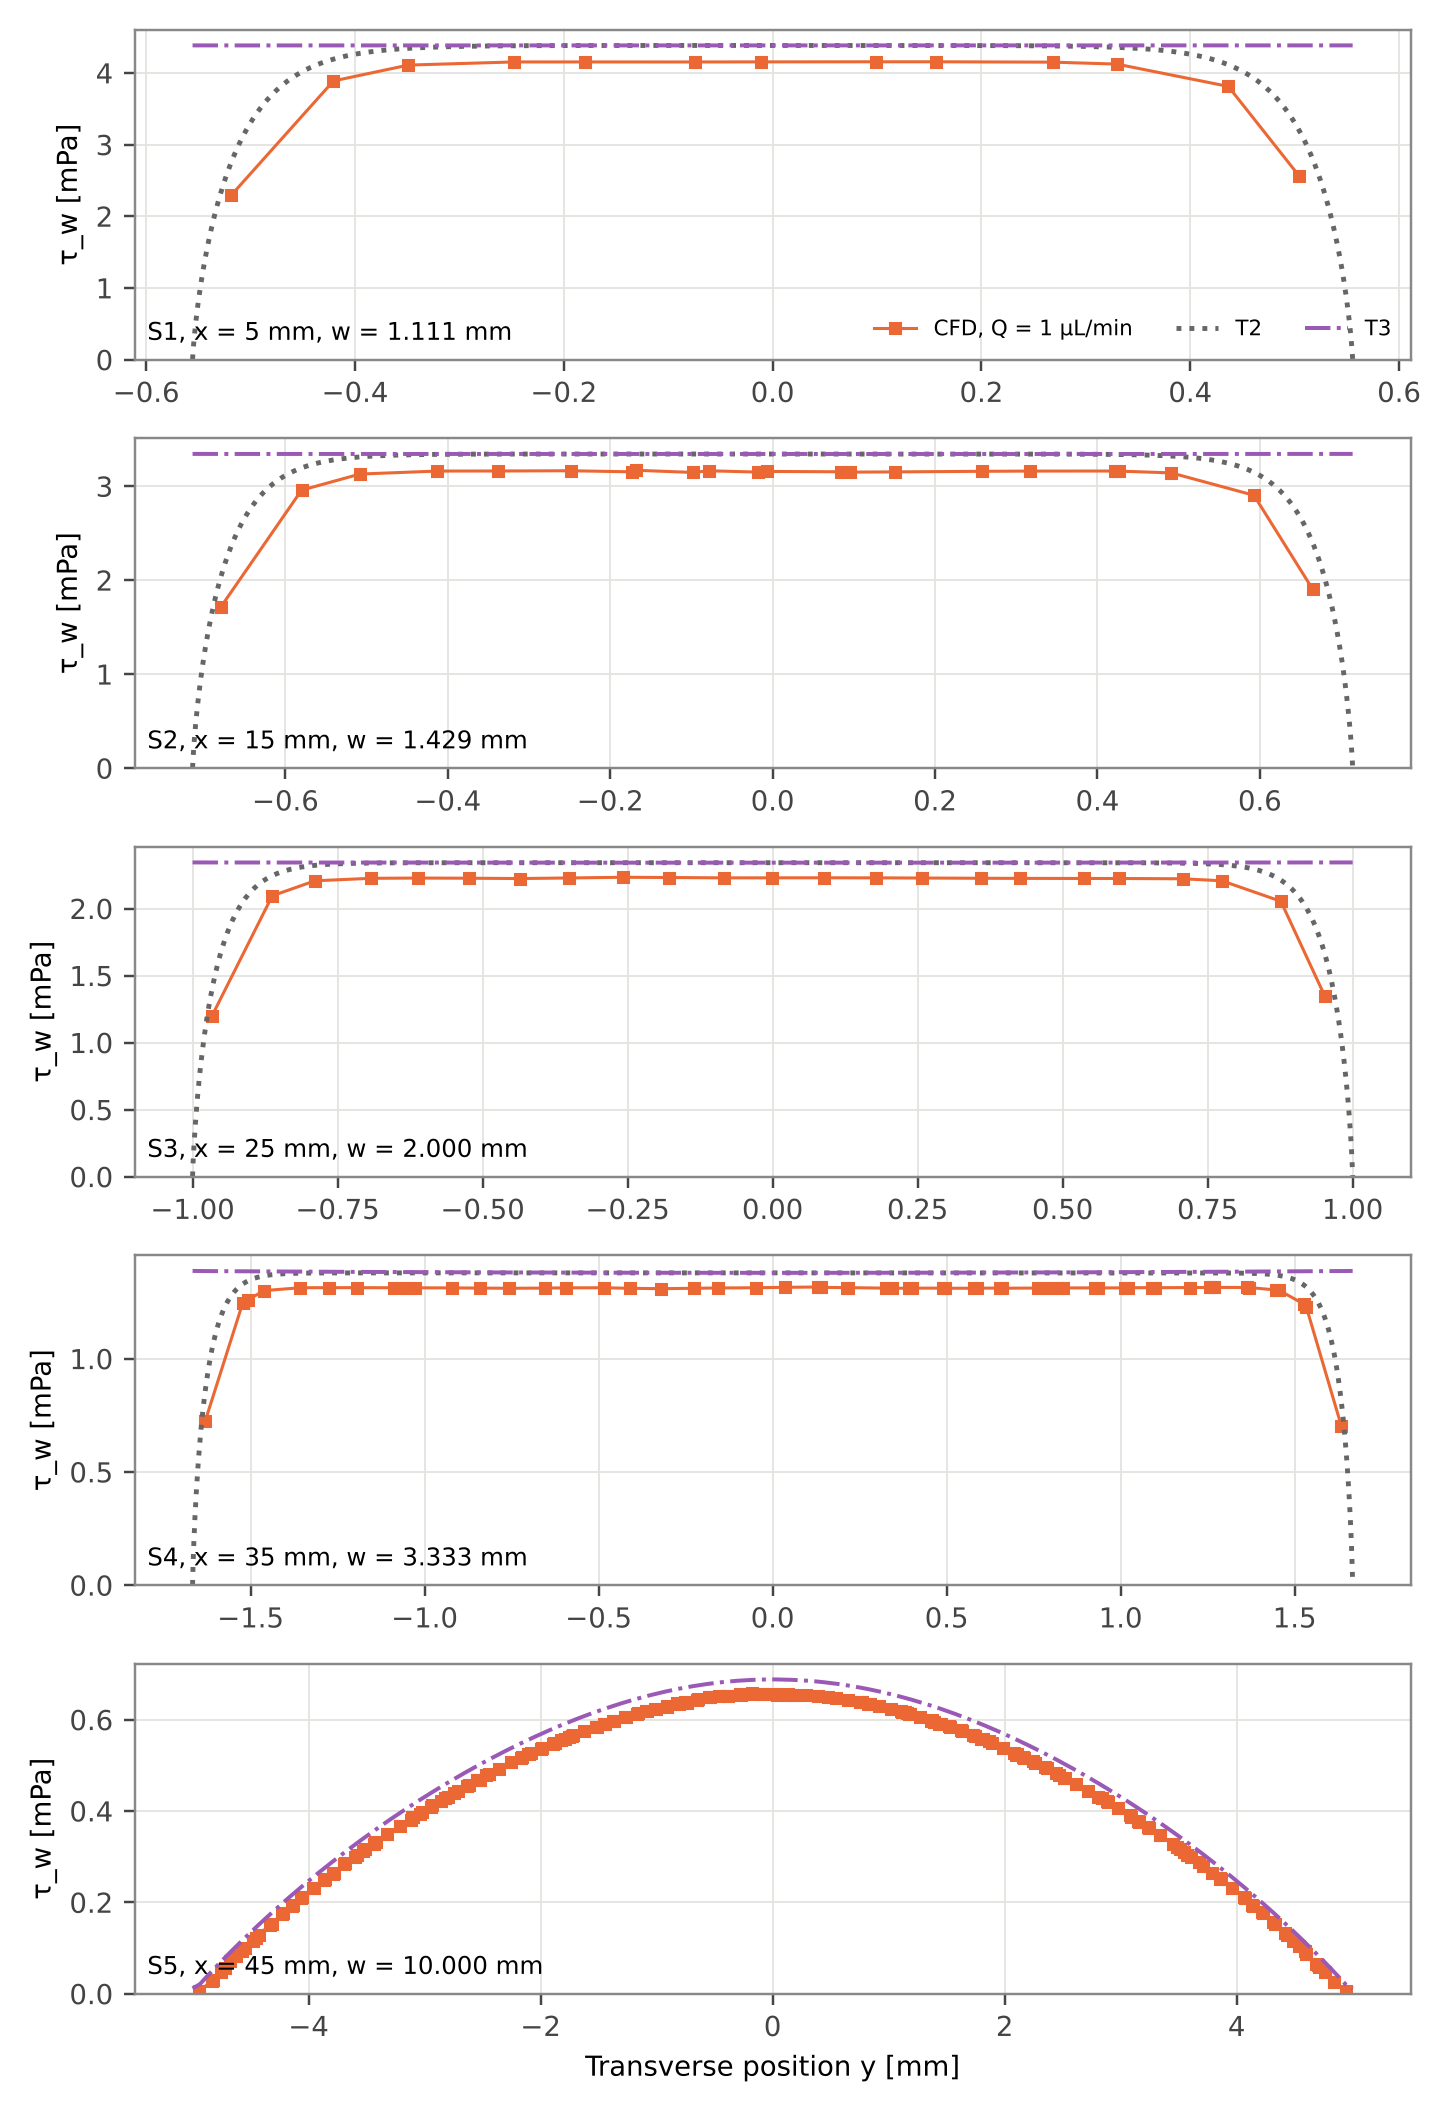
\includegraphics[width=\linewidth]{Fig22_transverse_shear_all_sections.png}
\caption{Floor shear across the width.}
\end{subfigure}\hfill
\begin{subfigure}[t]{0.49\linewidth}\centering
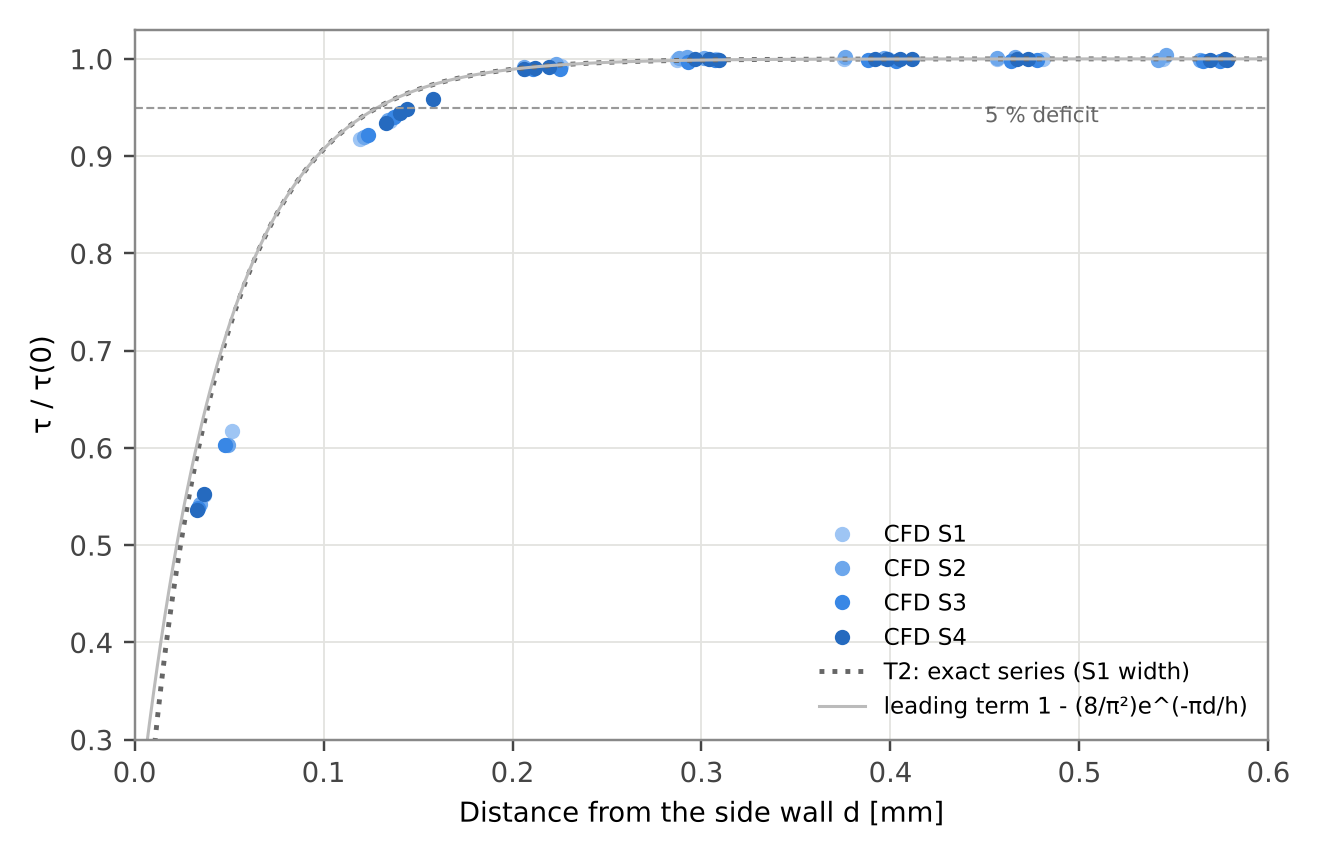
\includegraphics[width=\linewidth]{Fig25_sidewall_layer_collapse.png}
\caption{Against distance from the side wall.}
\end{subfigure}
\caption{Transverse floor shear at \SI{1}{\uLmin}. (a) S1--S4 show a plateau with side-wall layers about \SI{0.15}{mm} thick; S5 is dome-shaped. (b) S1--S4 collapse when plotted against distance from the wall; the theoretical \SI{5}{\percent} point is \SI{0.129}{mm}.}
\label{fig:transverse}
\end{figure}

\subsection{Internal consistency and the origin of the \texorpdfstring{\SI{-5}{\percent}}{-5\%} offset}

The CFD fields are internally consistent:
\begin{itemize}
\item the momentum balance $\taw=(h/2)|\dd p/\dd x|$ holds to within \SI{0.8}{\percent} at every station (\cref{tab:stations}); solved for the height, it gives $h=\SI{145(1)}{\micro\metre}$;
\item all interior quantities scale with $Q$ to within \SI{0.08}{\percent} over a 545-fold range; the only non-linearity, \SI{+0.7}{\percent}, is at the inlet face at \SI{120}{\uLmin};
\item the floor and lid shear agree to within \SIrange{0.1}{0.8}{\percent}.
\end{itemize}
The offset relative to T2/T3 is uniform in $x$ and identical at all three flow rates. A wrong $h$ cannot explain it, because $\Delta p\propto h^{-3}$ and $\taw\propto h^{-2}$ would give unequal offsets. A \SI{5}{\percent} flow deficit is unlikely, because the sampled peak velocity is only 1.2--\SI{3.4}{\percent} below theory, and this sampled value is itself a lower bound. The velocity field supports the same picture (\cref{fig:velocity}). Across the width it has a flat core and side-wall layers, as \cref{eq:rect} predicts, and the peak falls in proportion to $1/[wf]$. The decisive evidence is that the CFD peak velocity is \SIrange{1.6}{3.9}{\percent} \emph{above} $h^2|\dd p/\dd x|/8\mu$ (\cref{eq:parabola}), the maximum that an exact parabola with the CFD's own pressure gradient can reach. A discrete profile with too little wall friction behaves this way. This is consistent with about nine cells across the gap: a one-dimensional finite-volume estimate with nine layers already gives \SI{-2.4}{\percent}. Until the mesh study is done, the absolute CFD shear values should be considered probably about \SI{5}{\percent} low.

\begin{figure}[t]
\centering
\begin{subfigure}[t]{0.49\linewidth}\centering
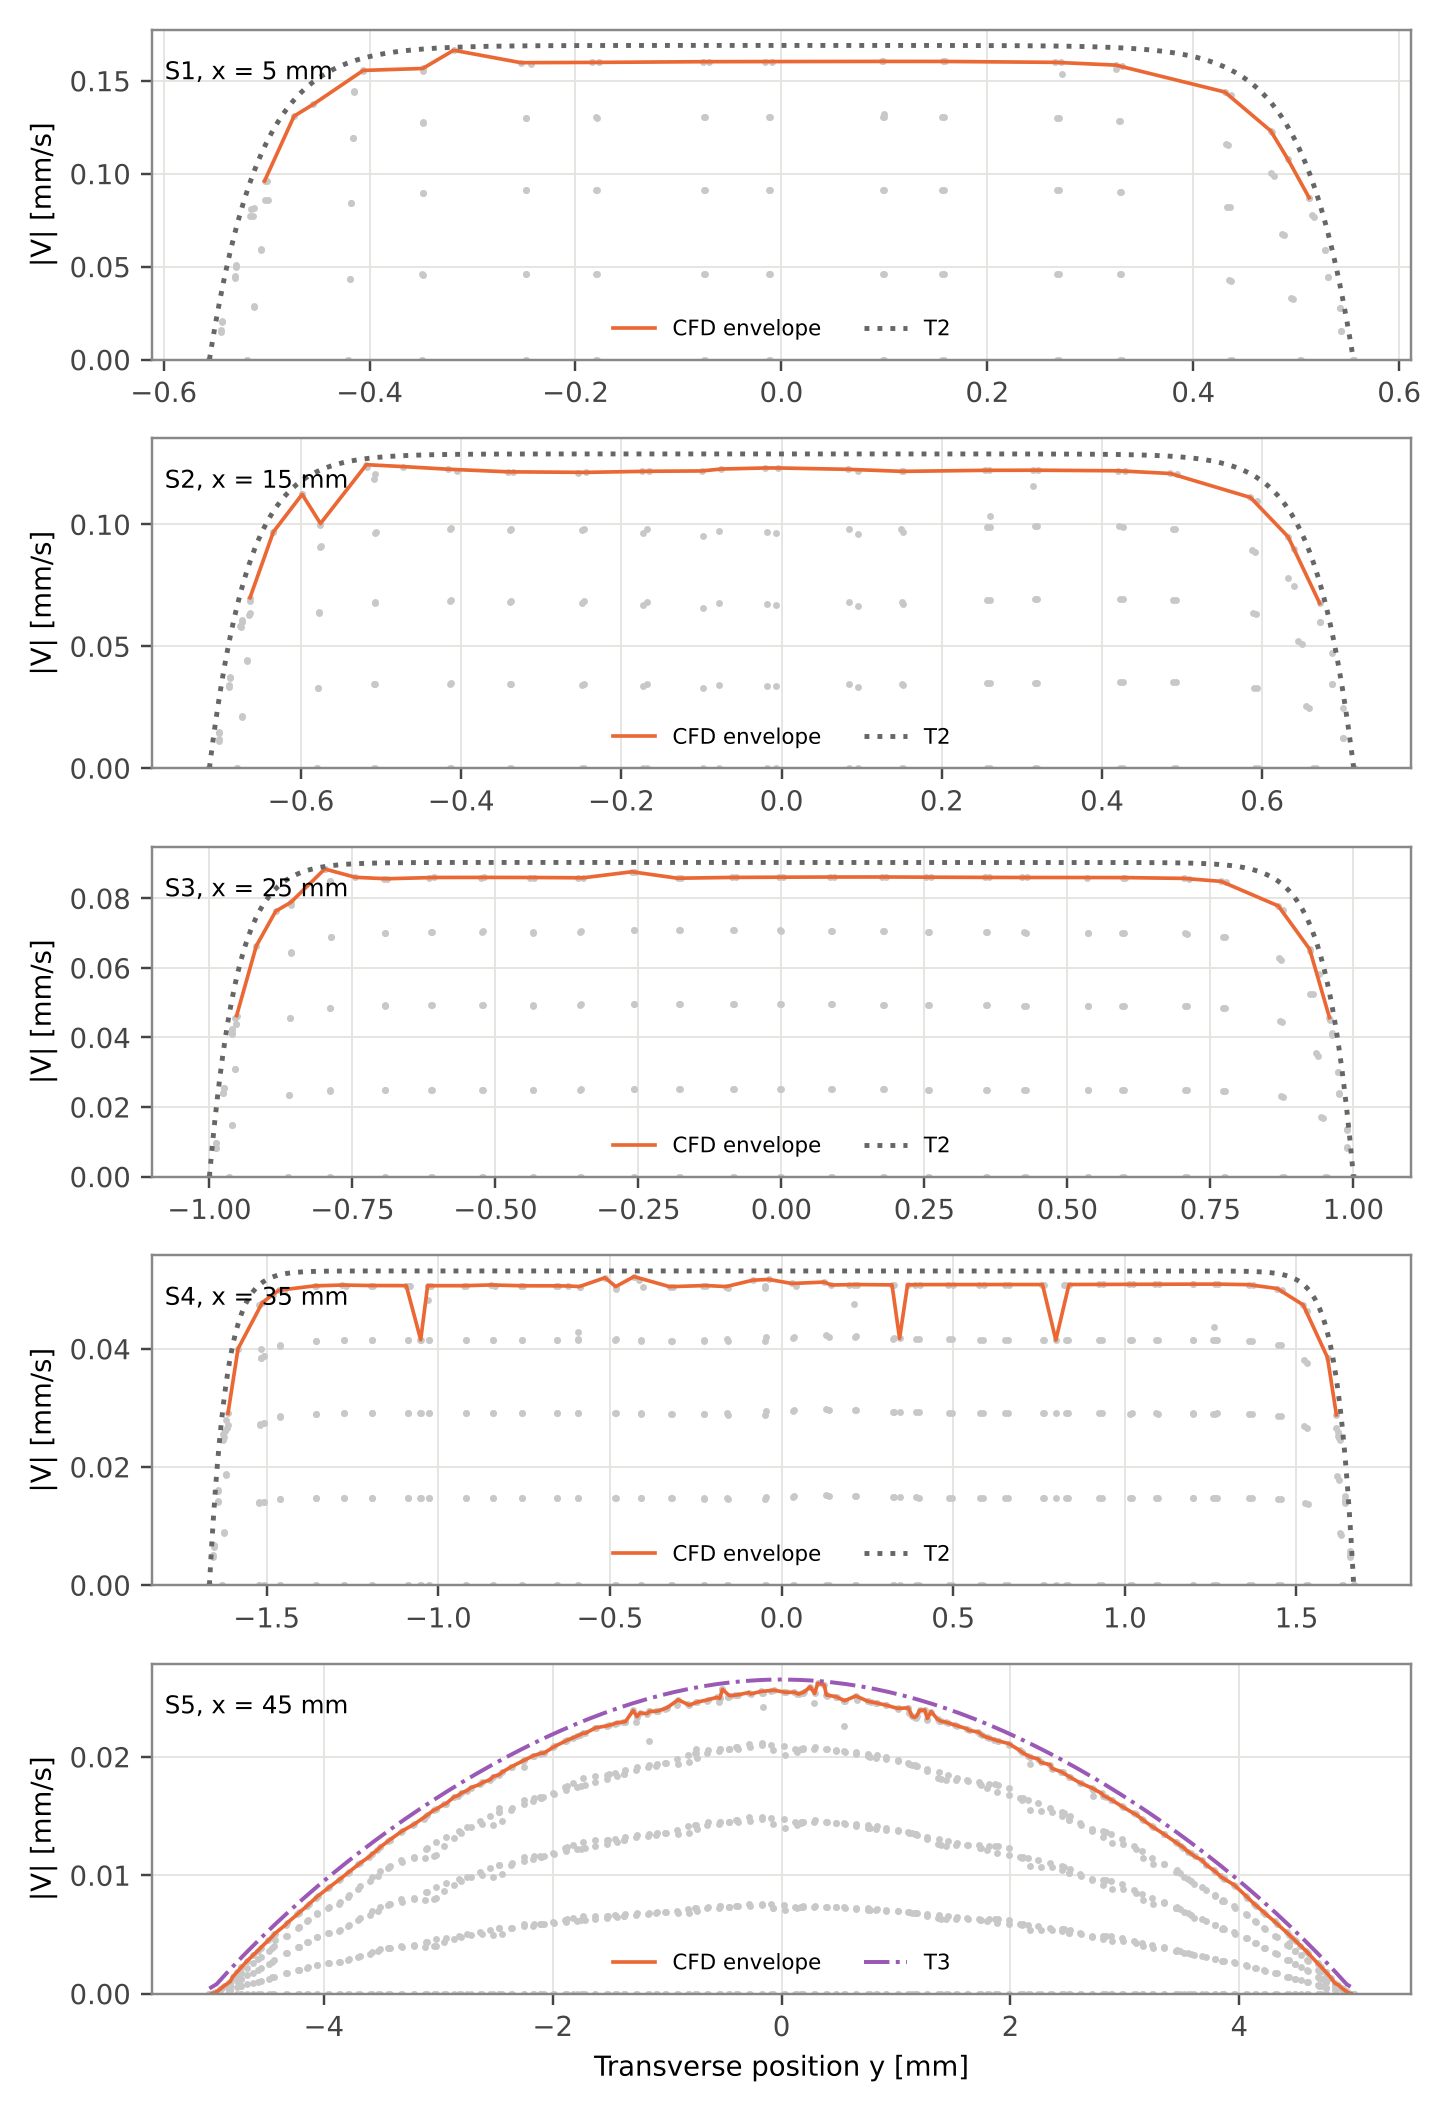
\includegraphics[width=\linewidth]{Fig33_transverse_velocity_all_sections.png}
\caption{Velocity magnitude across the width.}
\end{subfigure}\hfill
\begin{subfigure}[t]{0.49\linewidth}\centering
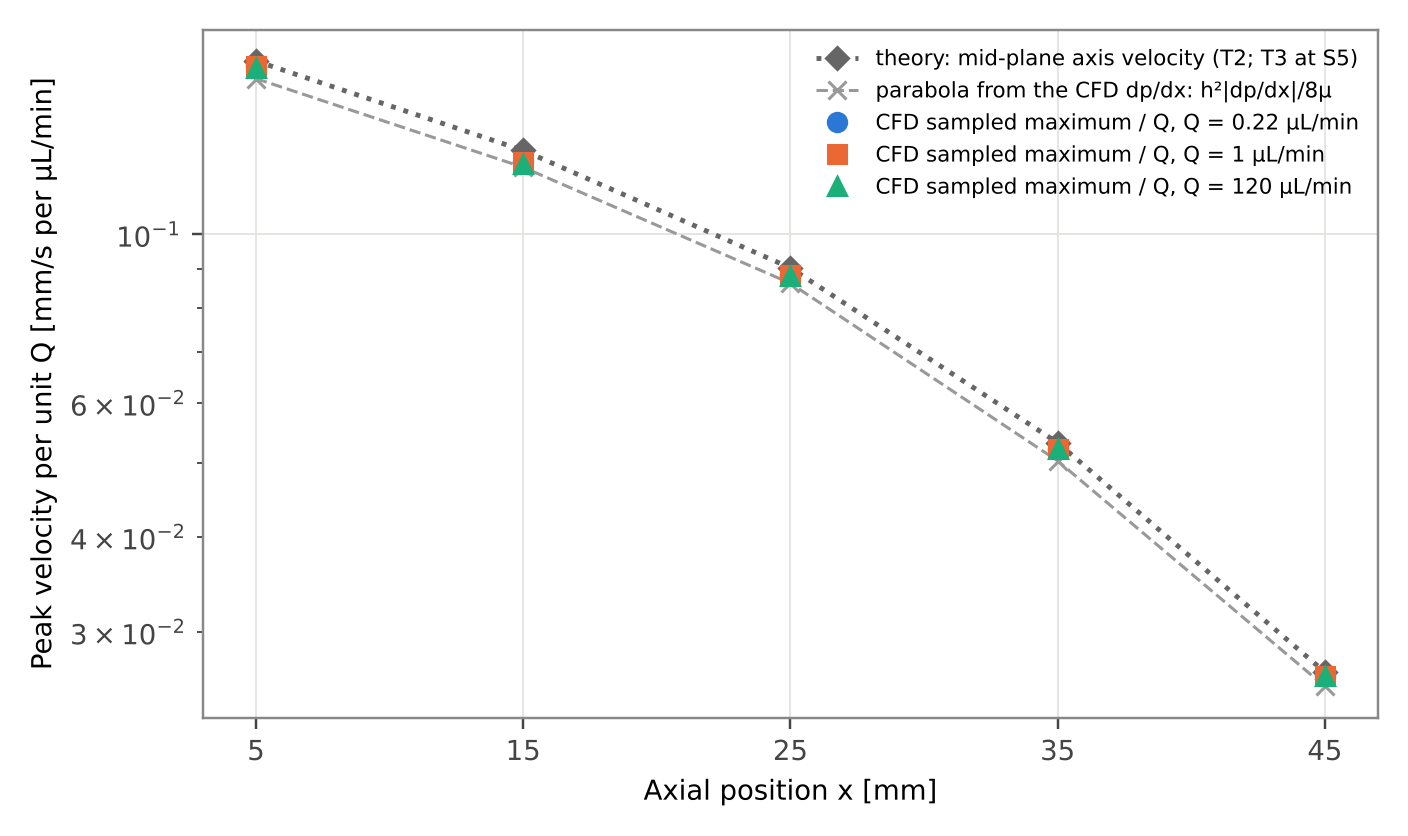
\includegraphics[width=\linewidth]{Fig35_peak_velocity_vs_x.png}
\caption{Peak velocity along the channel.}
\end{subfigure}
\caption{Velocity at the stations (\SI{1}{\uLmin}). (a) Nodes at all heights plotted against $y$; the exports contain no $z$ coordinate. The upper envelope approximates the mid-plane profile. (b) Highest sampled velocity per unit $Q$ against the theoretical mid-plane value: \SIrange{1.2}{3.4}{\percent} below it.}
\label{fig:velocity}
\end{figure}

\begin{table}[t]
\centering
\caption{Validation summary.}
\label{tab:matrix}
\small
\begin{tabularx}{\linewidth}{@{}p{0.31\linewidth}p{0.3\linewidth}X@{}}
\toprule
Quantity & Result & Status\\
\midrule
Published shear range, imaging zone & within a few \%; S3--S4 within \SI{2}{\percent} & consistent (semi-quantitative)\\
Shape of $p(x)$ and of $\taw(x)$ & within \SI{0.08}{\percent} / \SI{1}{\percent} of T3 & validated\\
Side-wall effect on $\taw$ & correct slope vs $h/w$ & validated\\
Uniform zone, side-wall layer & within node spacing of T2/T3 & consistent\\
Momentum balance, Stokes scaling & \SI{0.8}{\percent}; \SI{0.08}{\percent} & validated\\
Magnitude of $\taw$ and $\dd p/\dd x$ & \SI{5.2(4)}{\percent} below T2/T3 & deviating (probably mesh)\\
Velocity profile $u_x(z)$ & not exported & inconclusive\\
Mesh independence & one mesh only & inconclusive (study designed)\\
\bottomrule
\end{tabularx}
\end{table}

% =====================================================================
\section{Oxygen transport model}
\label{sec:oxygen}

\subsection{Formulation}

The oxygen concentration $C$ obeys $\partial_tC+\nabla\cdot(\bm uC)=\nabla\cdot(D\nabla C)+R$. We make the following assumptions:
\begin{itemize}
\item oxygen is dilute (mass fraction \num{6e-6}) and therefore does not affect the flow, so the coupling is one-way;
\item $D$ is constant;
\item $\nabla\cdot\bm u=0$;
\item the medium does not consume oxygen ($R=0$);
\item the system is at steady state: cultures last days, while the residence times are \SIrange{8}{4553}{s};
\item the \SIrange{5}{10}{\micro\metre} monolayer can be represented as a surface flux.
\end{itemize}
These give
\begin{equation}
\bm u\cdot\nabla C=D\nabla^2C,
\qquad D\left.\frac{\partial C}{\partial z}\right|_{0}=q=\qmax\frac{\Cbot}{\Km+\Cbot},
\label{eq:o2}
\end{equation}
with $C=\Csat$ at the inlet and zero diffusive flux at the outlet. Three cases bracket the lid:
\begin{itemize}
\item impermeable (IMP): $\partial C/\partial z=0$;
\item PDMS: $D\,\partial C/\partial z=\kp(\Csat-\Ctop)$;
\item saturated (SAT): $C=\Csat$.
\end{itemize}
The PDMS coefficient follows from steady permeation through a lid of thickness $t$ with Henry's law on the medium side: $\kp=P/(t\alpha)=\SI{5.65e-6}{m/s}$, for $P=800$ Barrer \citep{Merkel2000}, $t=\SI{5}{mm}$ and $\alpha=\SI{9.45e-6}{mol.m^{-3}.Pa^{-1}}$. The parameters are listed in \cref{tab:o2}. The uptake $\qmax=\rho_{\mathrm{cell}}\cdot\mathrm{OCR}$ combines the published seeding density with an \emph{illustrative} per-cell rate \citep{Wagner2011}. $\Km$ is a hepatocyte value \citep{Rotem1994}.

\begin{table}[t]
\centering
\caption{Oxygen parameters and dimensionless groups ($\bar U_0=Q/w_1h$, $A_{\mathrm{cells}}=\SI{115.13}{mm^2}$).}
\label{tab:o2}
\small
\begin{tabular}{@{}lll@{}}
\toprule
Parameter & Value & Source\\
\midrule
$D$ & \SI{3.0e-9}{m^2/s} & water, \SI{37}{\celsius} \citep{HanBartels1996}\\
$\Csat$ & \SI{0.178}{mol/m^3} & $1.26~\mu$M/mmHg $\times$ \SI{141}{mmHg} \citep{Wenger2015}\\
$\qmax$ & \SI{4e-8}{mol.m^{-2}.s^{-1}} (range 0.5--\num{50e-8}) & \SI{2e5}{cells/cm^2} \citep{Delon2020} $\times$ \SI{20}{amol/s} (illustrative)\\
$\Km$ & \SI{6.3e-4}{mol/m^3} (\SI{0.5}{mmHg}) & \citep{Rotem1994}\\
$\kp$ & \SI{5.65e-6}{m/s} & derived\\
\bottomrule
\end{tabular}

\vspace{2mm}
\begin{tabular}{@{}llccc@{}}
\toprule
Group & Meaning & 0.22 & 1 & 120 \ulmin\\
\midrule
$\Pe_h=\bar U_0h/D$ & convection vs diffusion across gap & 1.22 & 5.56 & 667\\
$\Da_w=\qmax h/D\Csat$ & uptake vs diffusion across gap & 0.011 & 0.011 & 0.011\\
$\Da_{\mathrm{conv}}=\qmax A_{\mathrm{cells}}/Q\Csat$ & uptake vs convective supply & \textbf{7.06} & \textbf{1.55} & 0.013\\
$\Phi=\kp\Csat/\qmax$ & lid supply vs uptake & 25.1 & 25.1 & 25.1\\
$t_{\mathrm{res}}=A_{\mathrm{cells}}h/Q$ & residence time [s] & 4553 & 1002 & 8.3\\
\bottomrule
\end{tabular}
\end{table}

\Cref{fig:groups} shows how the regime changes with flow rate. The uptake exceeds the convective supply ($\Da_{\mathrm{conv}}>1$) below \SI{1.55}{\uLmin}, while diffusion across the gap is always fast ($\Da_w\ll1$).

\begin{figure}[t]
\centering
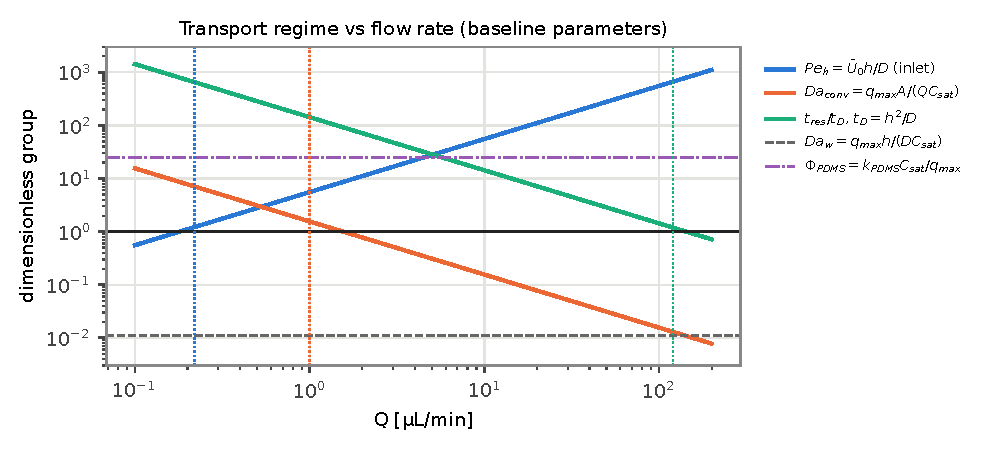
\includegraphics[width=0.78\linewidth]{oxygen_dimensionless_groups.pdf}
\caption{Oxygen transport groups against flow rate (baseline parameters). The vertical lines mark the three simulated flow rates.}
\label{fig:groups}
\end{figure}

\subsection{Reduction to a cup-mixing balance}

The terms of \cref{eq:o2} compare as follows. Axial diffusion is $O(h/\ell)^2$ relative to diffusion across the gap, and convection is $O(\Pe_h h/\ell)$, which is 0.004 and 0.016 at the culture flow rates. The concentration across the gap therefore equilibrates locally, while its axial variation is governed by the overall balance. Integrating \cref{eq:o2} over a cross-section, with the cup-mixing concentration $\Cb=Q^{-1}\iint u_xC\,\dd y\,\dd z$ and the side walls neglected, gives
\begin{equation}
Q\frac{\dd\Cb}{\dd x}=w(x)\,(N-q)
\quad\Longrightarrow\quad
Q\frac{\dd\Cb}{\dd A}=N-q,\qquad A(x)=\int_0^xw\,\dd x'=w_1L\ln\frac{L}{L-x},
\label{eq:cup}
\end{equation}
where $N$ is the supply through the lid. The geometry enters only through the upstream cell area $A(x)$. In the hyperbolic channel this area grows faster than $x$: at \SI{40}{mm} it is twice that of a straight channel of width $w_1$. The widening that lowers the shear downstream also makes the downstream cells feed on medium that has already passed over the most cells.

\paragraph{Exact closure across the gap.} With a parabolic $u_x$ and a locally fully developed profile, $D\,\partial^2C/\partial z^2=u_x\,\dd\Cb/\dd x$, with fluxes $q$ at $\eta=z/h=0$ and $N$ at $\eta=1$. Integrating twice,
\begin{equation}
C(\eta)=\Cbot+\frac hD\Big[q\eta+(N-q)\Big(\eta^3-\frac{\eta^4}{2}\Big)\Big].
\end{equation}
Flow-weighted averaging gives the wall-to-bulk relations
\begin{equation}
\Cb-\Cbot=\frac hD\Big(\frac{13}{35}q+\frac{9}{70}N\Big),\qquad \Ctop-\Cb=\frac hD\Big(\frac{13}{35}N+\frac{9}{70}q\Big).
\label{eq:closure}
\end{equation}
These reproduce the classical Sherwood numbers $70/13=5.385$ (one wall with flux, the other impermeable) and $140/17=8.235$ (equal flux at both walls) \citep{ShahLondon1978}. The drop across the gap is at most $qh/D=\Da_w\Csat\approx\SI{1.1}{\percent}$ of saturation. Diffusion across the gap is therefore never limiting (\cref{fig:o2z}).

\begin{figure}[t]
\centering
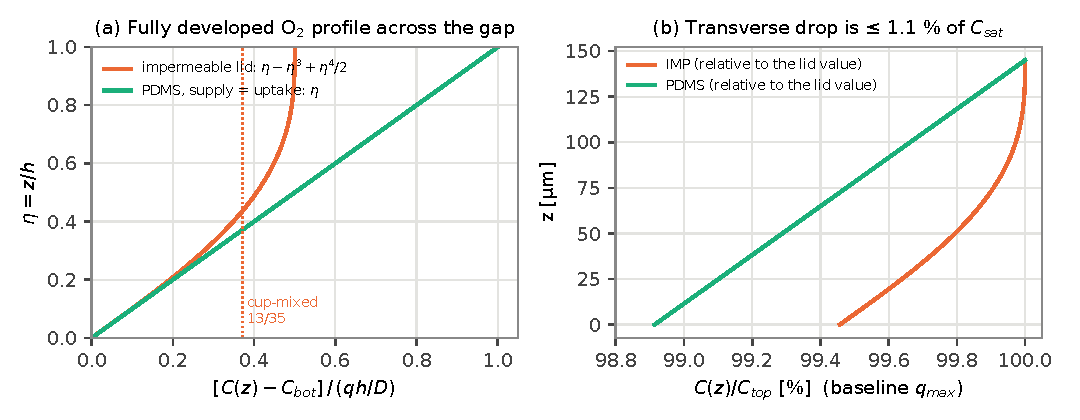
\includegraphics[width=0.82\linewidth]{oxygen_transverse_profile.pdf}
\caption{Fully developed oxygen profile across the gap. (a) Dimensionless profiles for an impermeable lid ($\eta-\eta^3+\eta^4/2$) and for a PDMS lid in equilibrium (linear). (b) For the baseline uptake, the variation across the gap is at most \SI{1.1}{\percent}.}
\label{fig:o2z}
\end{figure}

\subsection{Closed-form solutions}

Because $\Csat/\Km=283$, the uptake is zero order ($q=\qmax$) until $\Cbot<0.03\,\Csat$.

\paragraph{Impermeable lid.} With $N=0$, \cref{eq:cup} integrates to
\begin{equation}
\frac{\Cbot(x)}{\Csat}=1-\Da_{\mathrm{conv}}\frac{A(x)}{A_{\mathrm{cells}}}-\frac{13}{35}\Da_w,
\qquad
x_{\mathrm{crit}}=L\Big[1-\exp\Big(-\frac{Q\Csat}{\qmax w_1L}\Big)\Big],
\qquad
Q_{\min}=\frac{\qmax A_{\mathrm{cells}}}{\Csat}.
\label{eq:imp}
\end{equation}
The floor becomes anoxic beyond $x_{\mathrm{crit}}=\SI{13.9}{mm}$ at \SI{0.22}{\uLmin} and \SI{38.7}{mm} at \SI{1}{\uLmin}. Convection alone supplies the whole floor only if $Q>Q_{\min}=\SI{1.55}{\uLmin}$. Neither $h$ nor $D$ appears in $x_{\mathrm{crit}}$. Beyond $x_{\mathrm{crit}}$ the uptake is first order, with uptake and diffusion acting as two resistances in series, $k_{\mathrm{eff}}^{-1}=\Km/\qmax+\tfrac{13}{35}h/D$. The concentration then decays as $\exp[-k_{\mathrm{eff}}(A-A_c)/Q]$, over a length of about \SI{0.1}{mm}, so the transition to anoxia is sharp.

\paragraph{PDMS lid.} Eliminating $\Ctop$ with \cref{eq:closure} gives $N=k'[(\Csat-\Cb)-\tfrac{9}{70}\tfrac hD\qmax]$, with $k'=\kp/(1+\tfrac{13}{35}\Bi)$ and $\Bi=\kp h/D=0.27$. \Cref{eq:cup} then becomes linear, and its solution relaxes exponentially in $A$:
\begin{equation}
\Cb=\Cb_\infty+(\Csat-\Cb_\infty)e^{-k'A/Q},\qquad
\frac{C_{\mathrm{bot},\infty}}{\Csat}=1-\frac1\Phi-\Da_w=0.949 .
\label{eq:pdms}
\end{equation}
In the equilibrium state the lid supplies exactly what the cells consume and the profile across the gap is linear. The equilibrium is independent of $Q$ and of the geometry, and it is reached within $x^*=0.7$ and \SI{3.1}{mm} at 0.22 and \SI{1}{\uLmin}. For a saturated lid, $C_{\mathrm{bot},\infty}/\Csat=1-\Da_w=0.989$.

\paragraph{Reduced-order (1.5-D) model.} The general case, with Michaelis--Menten uptake and any lid, is obtained by integrating \cref{eq:cup} numerically with the closure \cref{eq:closure}. The local fluxes are solved at each $x$ (Brent's method plus Runge--Kutta). The integrated uptake balances the oxygen lost by the flow to within \SI{0.03}{\percent}. In the zero-order range the solution coincides with \cref{eq:imp,eq:pdms}: for example, 0.9496 against 0.9494 at \SI{45}{mm} for \SI{1}{\uLmin} with a PDMS lid. The concentration entrance length is 0.008, 0.04 and \SI{4.4}{mm} at the three flow rates. In this entrance region the fully developed closure over-predicts the depletion by at most \SI{0.4}{\percent} of saturation, which is conservative.

% =====================================================================
\section{Oxygen results}

\Cref{fig:o2axial} and \cref{tab:o2res} summarise the predictions. All of them are model results.

\begin{figure}[t]
\centering
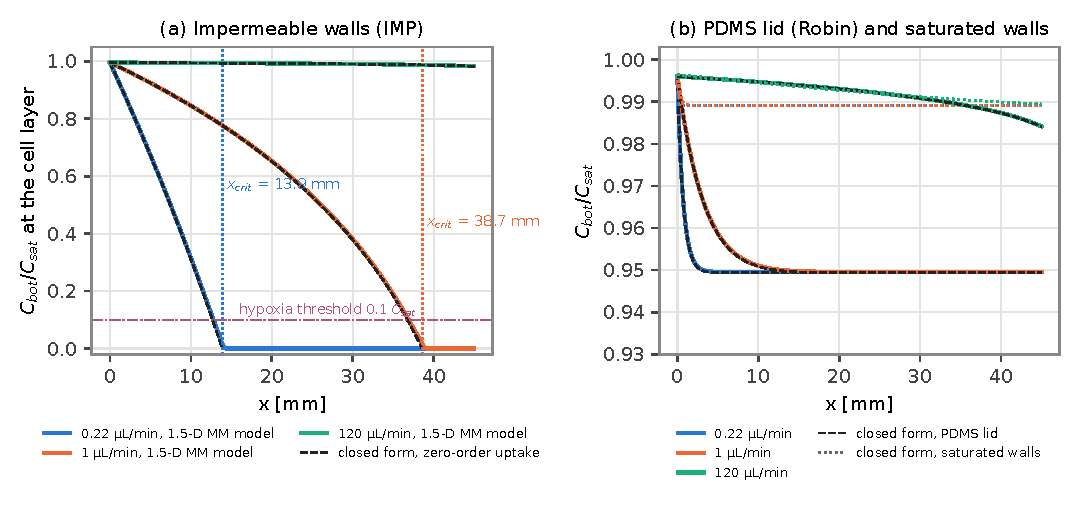
\includegraphics[width=\linewidth]{oxygen_axial_profiles.pdf}
\caption{Oxygen at the cell layer along the channel. Coloured lines: 1.5-D model with Michaelis--Menten uptake. Dashed: closed forms, \cref{eq:imp,eq:pdms}. Dotted: saturated lid. (a) Impermeable walls: anoxia beyond $x_{\mathrm{crit}}$ at 0.22 and \SI{1}{\uLmin}. (b) PDMS lid: rapid relaxation to $0.949\,\Csat$ at all flow rates.}
\label{fig:o2axial}
\end{figure}

\begin{table}[t]
\centering
\caption{Predicted oxygen at the cell layer, $\Cbot/\Csat$ (1.5-D model, baseline parameters). Window: $5\le x\le\SI{40}{mm}$. Hypoxic: fraction of the window area with $\Cbot<0.1\,\Csat$.}
\label{tab:o2res}
\small
\resizebox{\linewidth}{!}{%
\begin{tabular}{@{}llcccccccc@{}}
\toprule
$Q$ [\ulmin] & Lid & S1 & S2 & S3 & S4 & S5 & Mean (window) & Hypoxic & Demand met\\
\midrule
0.22 & IMP & 0.675 & 0 & 0 & 0 & 0 & 0.050 & 0.87 & \SI{14}{\percent}\\
1 & IMP & 0.925 & 0.757 & 0.531 & 0.190 & 0 & 0.426 & 0.18 & \SI{64}{\percent}\\
120 & IMP & 0.995 & 0.994 & 0.992 & 0.989 & 0.983 & 0.991 & 0 & \SI{99.6}{\percent}\\
0.22, 1 & PDMS & 0.95--0.96 & 0.950 & 0.950 & 0.950 & 0.950 & 0.950 & 0 & \SI{99.6}{\percent}\\
all & SAT & $\ge0.989$ & & & & & 0.989--0.992 & 0 & \SI{99.6}{\percent}\\
\bottomrule
\end{tabular}}
\end{table}

\paragraph{The flow cannot feed the cells; the walls decide.} With impermeable walls, $\Da_{\mathrm{conv}}=7.1$ and 1.55 at the two culture flow rates, so the flow delivers only 14 and \SI{64}{\percent} of the maximum demand. The outlet medium is fully depleted, and \SI{87}{\percent} and \SI{18}{\percent} of the imaging window is hypoxic. At \SI{120}{\uLmin} the depletion is only \SI{1.3}{\percent}. Diffusion across the gap is never limiting ($\Da_w=0.011$), so the familiar P\'eclet number does not decide oxygen availability: $\Pe_h=1.2$ at \SI{0.22}{\uLmin}, yet most of the floor is anoxic. The controlling group is $\Da_{\mathrm{conv}}$. With a \SI{5}{mm} PDMS lid, the lid supplies 97--\SI{99}{\percent} of the oxygen consumed at the culture flow rates. The cells sit at $0.95\,\Csat$ everywhere.

\paragraph{Shear and oxygen are confounded without a permeable lid.} \Cref{fig:o2tau}a plots the oxygen at the cells against the local shear. With impermeable walls, every cell below about 0.008 (\SI{0.22}{\uLmin}) or \SI{0.010}{\dyncm} (\SI{1}{\uLmin}) is anoxic. These are precisely the low-shear cells the device was designed to study, so a shear-response experiment would be confounded by hypoxia. With PDMS, oxygen is uniform over the whole shear range.

\begin{figure}[t]
\centering
\begin{subfigure}[t]{0.38\linewidth}\centering
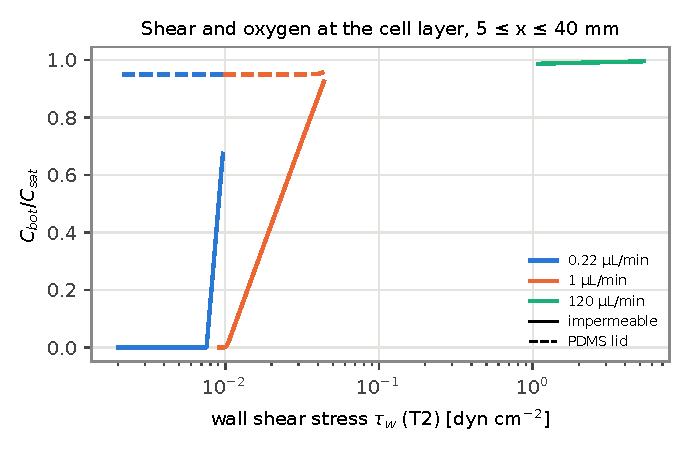
\includegraphics[width=\linewidth]{oxygen_vs_shear.pdf}
\caption{Oxygen against local shear.}
\end{subfigure}\hfill
\begin{subfigure}[t]{0.6\linewidth}\centering
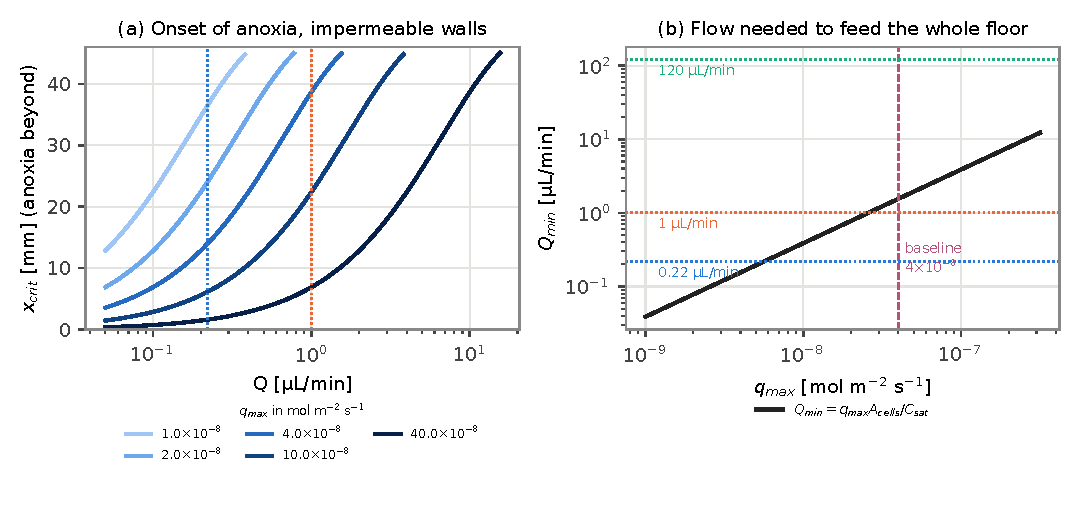
\includegraphics[width=\linewidth]{oxygen_design_map.pdf}
\caption{Design maps (impermeable walls).}
\end{subfigure}
\caption{(a) Oxygen at the cell layer against wall shear for $5\le x\le\SI{40}{mm}$. Solid lines: impermeable walls. Dashed lines: PDMS lid. (b) Onset of anoxia, $x_{\mathrm{crit}}$, against $Q$ for a range of $\qmax$, and the minimum flow rate $Q_{\min}$ against $\qmax$, both from \cref{eq:imp}.}
\label{fig:o2tau}
\end{figure}

\paragraph{Sensitivity.} The closed forms show which parameters matter. $\qmax$ dominates: over 0.5--\SI{50e-8}{mol.m^{-2}.s^{-1}}, $Q_{\min}$ ranges from 0.19 to \SI{19}{\uLmin} (\cref{fig:o2tau}b), and the PDMS equilibrium ranges from 0.994 to $0.37\,\Csat$. The PDMS equilibrium stays above $0.87\,\Csat$ for $\qmax\le\SI{1e-7}{mol.m^{-2}.s^{-1}}$. Changing $\Csat$ (0.167--0.200) moves $x_{\mathrm{crit}}$ by about \SI{1}{mm}. $D$ and $\Km$ have almost no effect. A lid with 600 Barrer or \SI{8}{mm} thickness lowers the equilibrium to 0.94 or $0.93\,\Csat$.

% =====================================================================
\section{Discussion}

\paragraph{Accuracy of the design formula.} Eq.~2 is accurate to about $\pm\SI{4}{\percent}$ for $x\lesssim\SI{40}{mm}$, but not for the reason a direct comparison suggests. It under-predicts the true axial shear by up to \SI{10}{\percent} near the inlet, because it neglects side-wall drag, and it fails at S5 because of the corner. Our CFD reproduces both effects with the correct form, while carrying a uniform offset that partly cancels the first. This is a general lesson for validation: close agreement between a simulation and a simple formula is not evidence that either is correct. Comparing the structure of the residual against a hierarchy of models (T1--T3) is what revealed the cancellation.

\paragraph{What oxygen modelling adds.} The flow analysis tells us which shear each cell feels. The oxygen analysis tells us whether shear is the \emph{only} variable. For an impermeable device at culture flow rates it is not. For the actual PDMS device the model predicts uniform oxygen at \SI{95}{\percent} of saturation, which would make the device sound for shear studies. This conclusion depends on two conditions: the lid must keep its permeability, and it must be exposed to air. Protein adsorption reduces PDMS permeability \citep{Mehta2007}, and immersing the device in water, which the protocol suggests to limit bubbles \citep{Delon2020}, adds a transport resistance. The design levers follow from \cref{eq:imp}. Since $\taw\propto Q/h^2$ while the supply scales with $Q$, doubling $h$ at constant shear allows four times the flow and cuts $\Da_{\mathrm{conv}}$ by four, at the cost of thicker side-wall layers. A thinner lid raises $\Phi$, and oxygen-enriched medium raises $\Csat$.

\paragraph{Limitations.} Both parts of the study have limitations.
\begin{enumerate}
\item \emph{Flow.} One mesh was run, with about nine layers across the gap, and the \SI{-5}{\percent} offset is attributed to discretisation but not yet demonstrated. The channel height and the lead-in were inferred rather than documented. The velocity exports lack $z$, so the parabola could not be tested. No mass balance was exported. The published results are available only as ranges.
\item \emph{Oxygen.} $\qmax$ and $\Km$ are illustrative. The model is steady and does not resolve the side-wall layers, where the slower fluid will deplete faster than predicted with impermeable walls. The PDMS is represented by a steady Robin coefficient. There is no oxygen CFD and no oxygen measurement.
\end{enumerate}
The next steps are: (i) the planned three-mesh GCI study at \SI{1}{\uLmin}; (ii) exports of $u_x(z)$, the floor shear alone, and the mass balance; (iii) the prepared Fluent oxygen case (a user-defined scalar with Michaelis--Menten and PDMS fluxes as user-defined functions), starting with a sign and mass-balance test; and (iv) measured uptake rates and on-chip oxygen sensing.

% =====================================================================
\section{Conclusions}

\begin{enumerate}
\item The widening Hele-Shaw chip operates in the Stokes regime at 0.22--\SI{120}{\uLmin}. Pressure, shear and velocity scale with $Q$ to within \SI{0.08}{\percent}, and $\Delta p=\SI{1.657}{Pa}$ per \ulmin.
\item The published shear ranges and imaging zones (at S3--S4) of Delon \emph{et al.}\ are reproduced.
\item The design formula agrees with the CFD to within $\pm\SI{3.3}{\percent}$ at S1--S4, partly because the side-wall drag it omits (up to \SI{+9}{\percent}) cancels a uniform \SI{-5}{\percent} CFD offset. The formula fails at the outlet corner (\SI{+46.5}{\percent} at S5), which a two-dimensional Hele-Shaw model captures to within \SI{1}{\percent} in shape.
\item The shear is uniform within $\pm\SI{5}{\percent}$ over \SI{70}{}--\SI{91}{\percent} of the width at S1--S4, bounded by side-wall layers about \SI{0.15}{mm} thick that scale with $h$. Imaging should use the centre of S2--S4.
\item Oxygen transport depends on the geometry only through $A(x)=w_1L\ln[L/(L-x)]$. With impermeable walls, convection cannot feed the cells below \SI{1.55}{\uLmin}, and the low-shear region becomes anoxic. A \SI{5}{mm} PDMS lid is predicted to keep the cells at $0.95\,\Csat$. Oxygen availability is therefore set by the walls and the uptake rate, not by the flow. These predictions still need to be tested by oxygen CFD and measurement.
\end{enumerate}

\paragraph{Data availability.} The raw Fluent exports, processed tables, scripts and an extended 78-page technical report (with full derivations, all 41 flow figures and a complete list of missing or assumed information) are provided with this paper.

\bibliographystyle{unsrtnat}
\bibliography{references}

\end{document}
